\documentclass[conference]{IEEEtran}
\IEEEoverridecommandlockouts

\usepackage{cite}
\usepackage{amsmath,amssymb,amsfonts}
\usepackage{algorithm}
\usepackage{algorithmic}
\usepackage{graphicx}
\usepackage{textcomp}
\usepackage{xcolor}
\usepackage{booktabs}
\usepackage{multirow}
\usepackage{url}
\usepackage{balance}

% Hyperref for interactive PDF links ([1] -> reference entry redirect, Fig. 1 -> figure redirect)
\usepackage[colorlinks=true, linkcolor=blue, citecolor=blue, urlcolor=blue, hypertexnames=false]{hyperref}

\def\BibTeX{{\rm B\kern-.05em{\sc i\kern-.025em b}\kern-.08em
    T\kern-.1667em\lower.7ex\hbox{E}\kern-.125emX}}

\begin{document}

% \title{FedRouteAI: Adaptive Federated Learning for Resilient\\
% Edge-Based Traffic Anomaly Detection}

% \author{
% \IEEEauthorblockN{Moguloju Abhiram\IEEEauthorrefmark{1},
% Rajulapudi Rohith\IEEEauthorrefmark{1}, and
% Segu Jyothsna\IEEEauthorrefmark{1}}
% \IEEEauthorblockA{\IEEEauthorrefmark{1}\textit{Department of Computer Science and Engineering (Data Science)}\\
% \textit{B V Raju Institute of Technology}, Narsapur, Telangana, India\\
% \{moguloju.abhiram, 23211a67a0, jyothsna.segu\}@bvrit.ac.in}
% }
\title{FedRouteAI: Adaptive Federated Learning for Resilient
Edge-Based Traffic Anomaly Detection}

\author{
\IEEEauthorblockN{Moguloju Abhiram, Rajulapudi Rohith, Segu Jyothsna}
\IEEEauthorblockA{
\textit{Department of Computer Science and Engineering (Data Science)}\\
\textit{B V Raju Institute of Technology}, Narsapur, Medak,  502313, Telangana, India\\
% Narsapur, Medak, 502313, Telangana, India
\{moguloju.abhiram, rohithrajulapudi and jyothsna.segu\}@gmail.com
}
}

\maketitle

\begin{abstract}
Modern Intelligent Transportation Systems (ITS) heavily rely on centralized machine learning architectures that require the continuous transmission of privacy-sensitive geospatial telemetry. Although Federated Learning (FL) provides a decentralized alternative by training models directly on edge devices, deploying these models in real-world traffic environments introduces severe vulnerabilities. Edge networks in particular are prone to dropped sensory data and extreme Out-Of-Distribution (OOD) inputs, which can cause unreliable or highly confident predictions. We introduce FedRouteAI, an end-to-end framework that pairs an AdaptiveFedAvg aggregation algorithm with a resilient inference pipeline. The architecture leverages a historical memory module to normalize live vehicular telemetry against localized, time-synchronized baselines, so that when real-time features drop out, the inference engine falls back on deterministic zero-imputation and dynamic out-of-distribution warnings rather than failing silently. On a multi-class synthetic geospatial dataset, the framework correctly identifies eight distinct traffic anomaly categories, and ablation studies show the adaptive aggregation mechanism converging to 82.2\% accuracy, comparable to standard federated averaging, while additionally supporting dynamic client weighting for heterogeneous edge environments.
\end{abstract}


\begin{IEEEkeywords}
Federated Learning, Intelligent Transportation Systems, Out-of-Distribution Detection, Edge Computing, Traffic Anomaly Classification, Adaptive Aggregation, Privacy-Preserving Machine Learning.
\end{IEEEkeywords}

\section{Introduction}

\subsection{Background}

The rapid deployment of Connected and Automated Vehicles (CAVs) has fundamentally transformed the landscape of Intelligent Transportation Systems (ITS). Modern ITS relies heavily on the continuous collection and analysis of vehicular telemetry, enabling complex machine learning architectures to predict traffic flows, manage congestion, and detect anomalous road events. However, this centralized paradigm demands the constant transmission of highly sensitive geospatial data---including high-frequency GPS trajectories, localized density metrics, and acceleration profiles---to cloud servers. Such bulk data aggregation exposes critical vulnerabilities regarding passenger privacy and location tracking, necessitating a shift toward decentralized processing architectures \cite{Zhang_2025}.

Federated Learning (FL) has emerged as the definitive framework for resolving the privacy-utility tradeoff in distributed edge networks \cite{Kairouz_2021}. By distributing the training process directly to the edge nodes (i.e., the vehicles or roadside units), FL allows statistical models to converge globally without requiring raw, privacy-sensitive data to leave the local device. In this architecture, edge nodes compute localized gradients using their immediate environmental data and transmit only the ephemeral model weight updates to a central aggregation server. This paradigm is rapidly becoming the standard for Vehicle-to-Everything (V2X) communication networks, theoretically offering scalable, privacy-preserving intelligence across the entire transportation grid.

\subsection{Motivation}

Despite the privacy advantages of Federated Learning, transitioning these models from controlled simulations to real-world edge deployments introduces significant challenges. Conventional FL algorithms, such as FedAvg, operate under the implicit assumption that the data distributions across all participating clients are relatively stable and complete. However, vehicular environments are inherently highly heterogeneous and volatile \cite{Lu_2024}.

In practical ITS deployments, edge devices---ranging from low-power roadside sensors to advanced on-board vehicle computers---frequently experience intermittent network connectivity, sensor degradation, and extreme environmental variations. These physical limitations directly translate into data abnormalities. When an autonomous vehicle encounters a faulty sensor or drops a telemetry packet, the resulting real-time feature vector becomes incomplete or severely skewed compared to the data distribution upon which the model was trained. Incomplete or out-of-distribution feature vectors can reduce the reliability of machine learning models during edge inference. Therefore, for an FL framework to be genuinely viable for mission-critical traffic anomaly detection, the inference pipeline itself must be engineered to withstand the volatile realities of edge data collection.

\subsection{Research Gap}

While existing literature has extensively explored federated optimization techniques to handle statistical heterogeneity, existing federated learning approaches for intelligent transportation systems primarily focus on privacy-preserving distributed training. Comparatively less attention has been given to maintaining reliable inference when deployed edge devices provide incomplete or out-of-distribution feature information. This creates a practical gap between successful model training and robust real-world deployment.

\subsection{Contributions}

Motivated by this gap, we propose FedRouteAI, a deployment-ready architecture that bridges federated training and practical edge inference. The specific contributions of this work are as follows:
\begin{enumerate}
    \item A federated learning framework for privacy-preserving multi-class traffic anomaly detection in intelligent transportation systems.
    \item A deployment-aware inference pipeline that maintains preprocessing consistency when feature information is incomplete or out-of-distribution.
    \item An adaptive federated aggregation mechanism designed to support decentralized traffic anomaly classification across heterogeneous edge nodes.
    \item An end-to-end implementation integrating edge inference, federated training, backend services, and visualization for practical deployment.
    \item A comprehensive experimental evaluation demonstrating the framework on a multi-class traffic anomaly dataset using standard classification metrics.
\end{enumerate}

\section{Related Work}

\subsection{Federated Learning in Intelligent Transportation Systems}

The integration of Federated Learning (FL) into Intelligent Transportation Systems has gained significant momentum as a solution to the inherent privacy risks associated with centralized traffic data collection. Recent literature extensively explores the application of FL across diverse vehicular contexts, including connected and automated vehicles (CAVs), traffic flow prediction, and edge-assisted route optimization \cite{Sanadi_2026}. For instance, frameworks such as FedGRU have demonstrated the ability to accurately forecast macroscopic traffic volumes without exposing the raw spatial-temporal trajectories of individual drivers \cite{Liu_2020}. Similarly, advanced architectures leveraging decentralized spatial-temporal networks (e.g., FedSTN) have been proposed to manage urban traffic heterogeneity across disparate geographical zones \cite{Yuan_2024, Zhang_2025}. These existing federated learning frameworks have primarily focused on privacy-preserving distributed training and communication efficiency, optimizing for bandwidth, privacy guarantees, or training accuracy. What reliable inference should look like once a client's own features arrive incomplete is left largely unaddressed.

\subsection{Traffic Anomaly Detection and Trajectory Analysis}

The detection of anomalies in vehicular networks has historically relied heavily on centralized data mining and deep learning architectures. Traditional methods often process raw, high-frequency GPS trajectories using grid-based clustering techniques to identify spatial deviations in real-time \cite{Raiyn_2014}. While effective in controlled settings, these trajectory-mining approaches generally struggle with the massive distance computation complexities inherent in large-scale urban grids \cite{Su_2019}. 

To capture complex spatial-temporal correlations, contemporary research has pivoted towards deep learning models. For example, centralized ResNet models equipped with attention mechanisms have successfully addressed the challenge of imbalanced incident data, achieving high accuracy in predicting anomalies across highway datasets \cite{El_Manaa_2022}. Furthermore, Spatial-Temporal Graph Neural Networks (ST-GNNs) have been proposed to map non-Euclidean road segments, forecasting traffic conditions and classifying congestion events with remarkable precision \cite{Gao_2023}. 

Despite their predictive power, many of these trajectory-based and graph-based approaches rely on processing high-dimensional GPS data or maintaining centralized spatial representations. Operating such architectures requires significant computational overhead, rendering them highly prohibitive for direct deployment on resource-constrained edge devices (e.g., roadside units or on-board computers), and transmitting the requisite spatial data to a central server fundamentally violates V2X privacy constraints. Their design goal is spatial prediction accuracy and graph computation efficiency; keeping anomaly classification reliable locally, without exposing raw trajectories, is not what they were built to solve.

\subsection{Edge Deployment Challenges and Out-of-Distribution Mitigation}

The deployment of deep learning models on intelligent edge devices is frequently bottlenecked by volatile operational environments. Research into adaptive federated optimization, such as FedYogi and FedAdam, has made significant strides in mitigating statistical heterogeneity by dynamically adjusting server-side learning rates \cite{Yang_2024}. Additionally, control algorithms for local updates have been developed to balance computational resource constraints at the network edge \cite{Wang_2020}. While these methods effectively address non-IID (Independent and Identically Distributed) training data divergence \cite{Lu_2024}, they generally operate under the assumption that inference-time inputs will adhere to the trained feature distributions. 

When deploying autonomous edge sensors, physical hardware faults and connectivity drops frequently result in extreme Out-of-Distribution (OOD) feature vectors. Many OOD detection techniques in computer vision and natural language processing rely on confidence calibration, such as temperature scaling (e.g., ODIN), or post-hoc scoring methods \cite{Shalev_2022}. However, their direct applicability to resource-constrained intelligent transportation deployments remains an active area of research. These traditional methods typically intervene only after the model has processed the malformed input, which can still lead to mathematical saturation and delayed response times on edge hardware. Across this body of work, the emphasis stays on server-side aggregation or post-hoc confidence scoring rather than on dynamic anomaly warnings and imputation at the point where features first arrive incomplete.

\subsection{Summary of Research Gap}

Collectively, the existing literature has made substantial progress in privacy-preserving federated learning, traffic anomaly detection, and edge intelligence. However, these research directions have largely evolved independently, leaving the challenge of maintaining reliable inference under incomplete feature availability in decentralized intelligent transportation systems comparatively underexplored. This observation motivates the deployment-aware methodology presented in the next section.

\section{Methodology}
\label{sec:methodology}

\subsection{Overall System Architecture}

FedRouteAI is an end-to-end, privacy-preserving federated learning framework for multi-class traffic anomaly detection. The system decouples inference from aggregation: all raw telemetry processing and local model training remain at the edge, and only 12.96\,KB model weight payloads are ever transmitted to the central server. Fig.~\ref{fig:architecture} illustrates the complete pipeline across six functional layers.

\begin{figure*}[t]
  \centering
  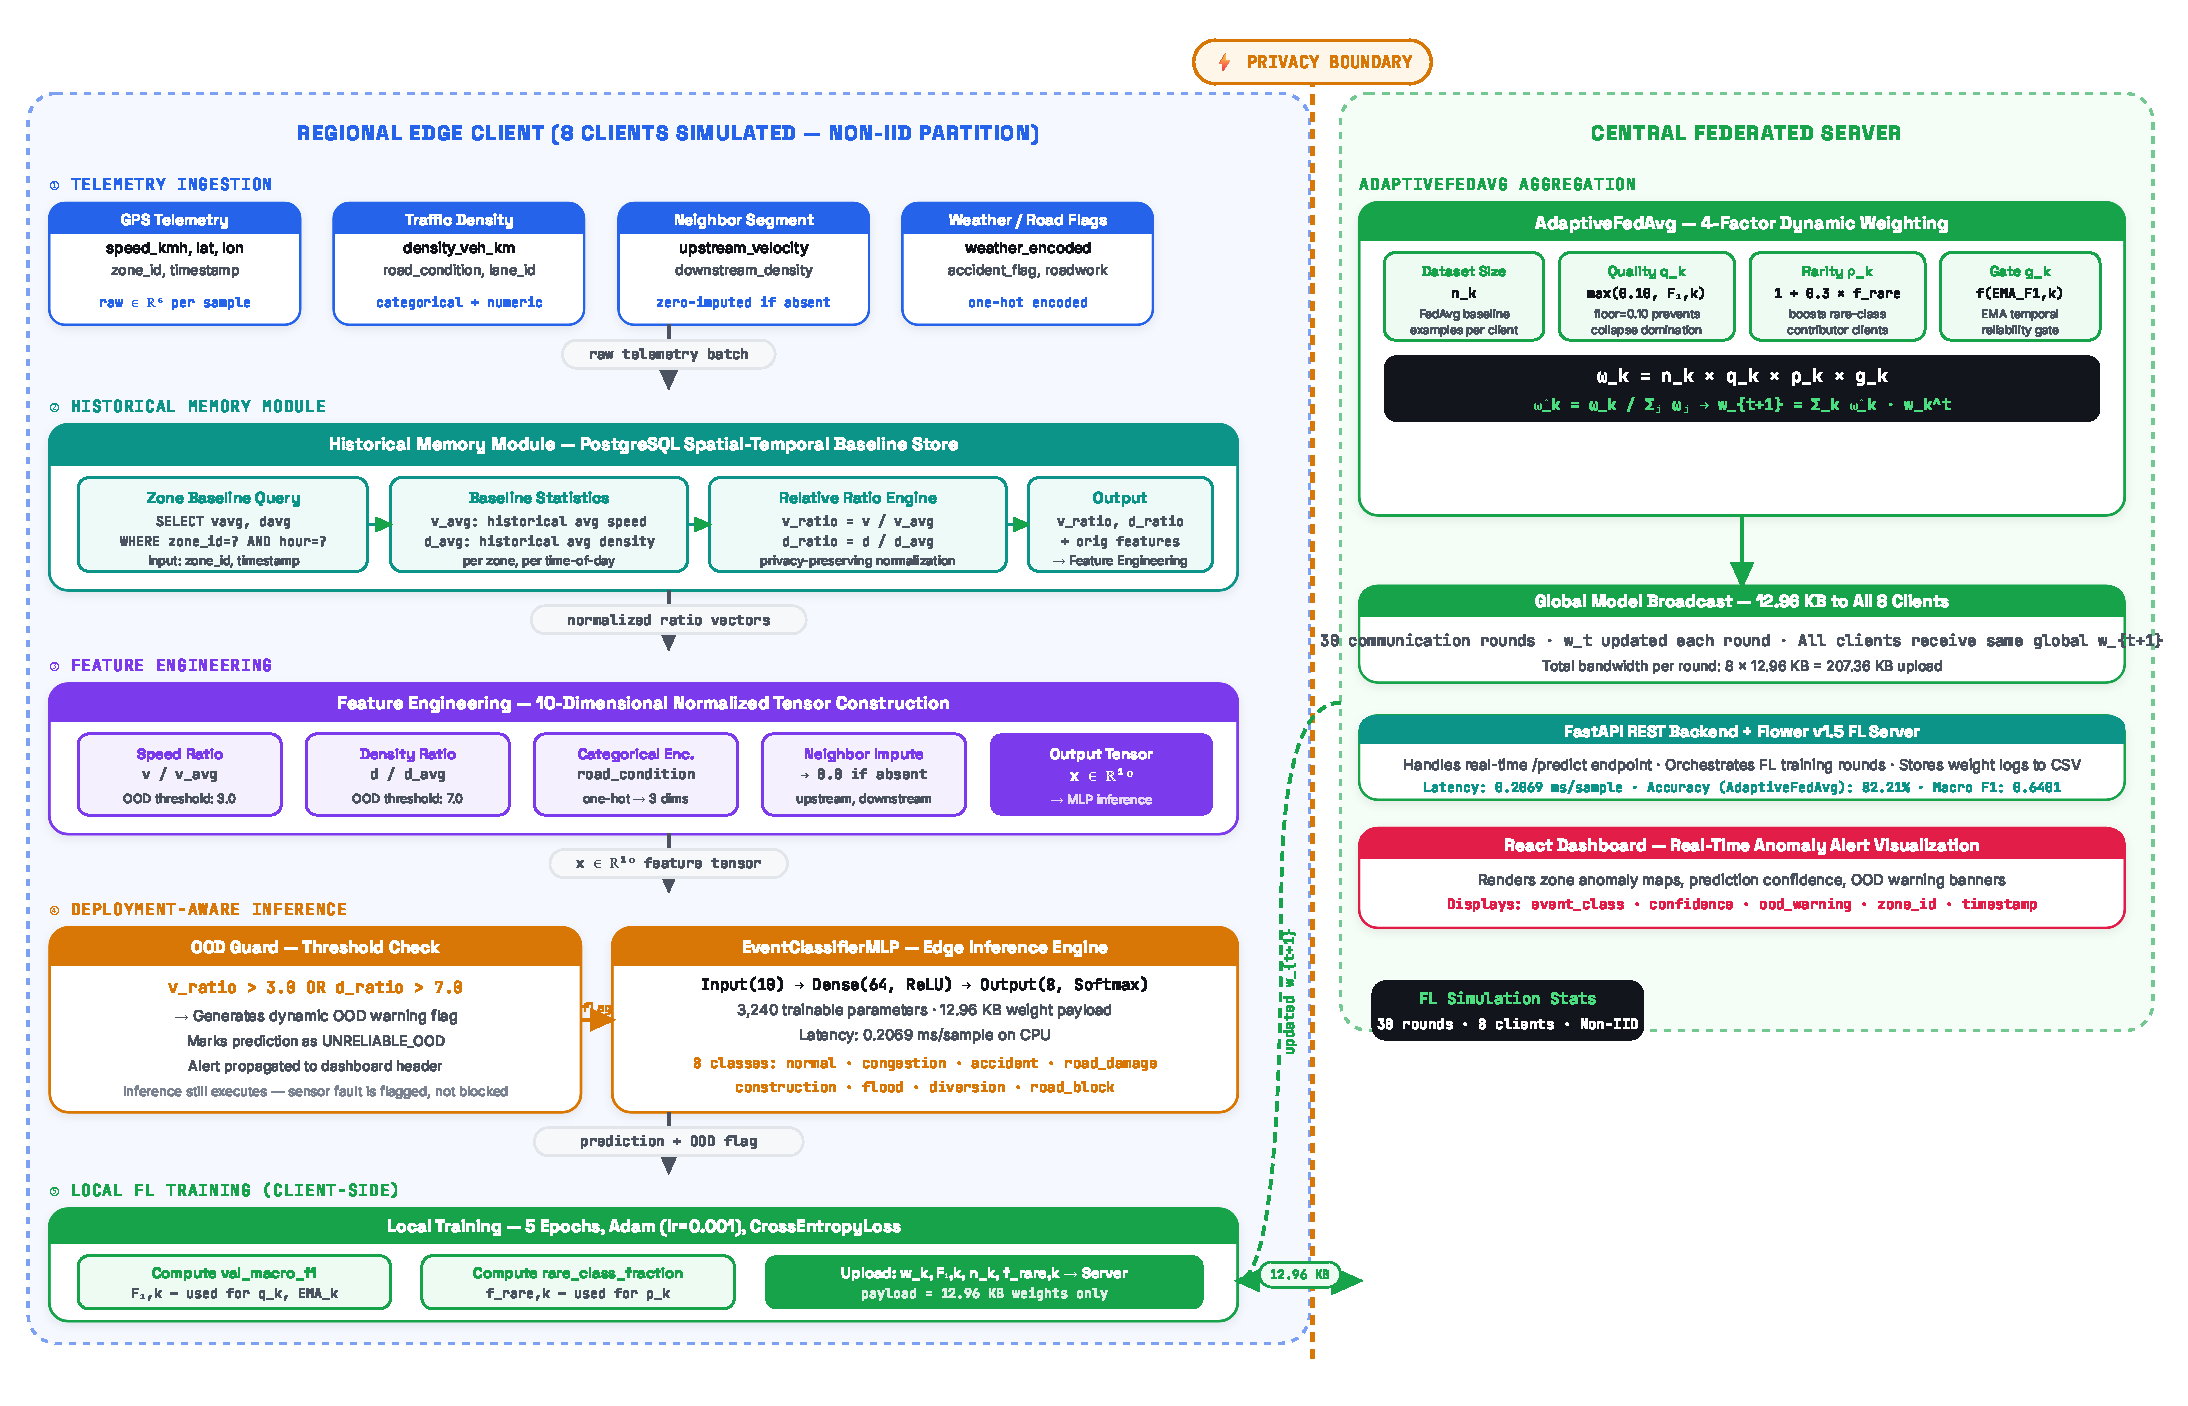
\includegraphics[width=0.95\textwidth]{figures/fig1_system_architecture}
  \caption{End-to-end FedRouteAI architecture. Raw GPS telemetry is processed entirely within the regional edge client (blue zone). Only 12.96\,KB model weights cross the privacy boundary (orange dashed line) to the central federated server (green zone). The six functional layers are: telemetry ingestion, Historical Memory normalization, feature engineering, deployment-aware MLP inference, AdaptiveFedAvg aggregation, and the React alerting dashboard.}
  \label{fig:architecture}
\end{figure*}

From an engineering perspective, the framework is orchestrated by a FastAPI backend interfacing with a PostgreSQL database for real-time telemetry ingestion. A React-based visualization dashboard displays live anomaly alerts across simulated geographical zones. The Flower~\cite{Beutel_2020} federated learning server manages communication rounds and model distribution.

The primary research contributions reside within two components: (1) a deployment-aware inference pipeline at the edge that handles real-world sensor degradation, and (2) an adaptive federated aggregation algorithm at the server that accounts for heterogeneous client quality.

\subsection{Historical Memory Module and Feature Engineering}

Directly classifying raw GPS telemetry poses privacy risks and generalization challenges, since absolute speed values differ across urban zone typologies (e.g., residential streets versus motorways). To resolve this, the \emph{Historical Memory Module}---implemented as a PostgreSQL spatial-temporal baseline store---maintains aggregated speed and density statistics per zone and per time-of-day slot~\cite{Chen_2016}.

Fig.~\ref{fig:historical_memory} details the module's internal dataflow. When an edge device records an instantaneous telemetry tuple $(v, d, \text{zone\_id}, t)$, the system queries the baseline store to retrieve historical averages $v_{avg}(\text{zone}, \text{hour})$ and $d_{avg}(\text{zone}, \text{hour})$. Two normalized relative ratios are then computed:

\begin{equation}
  v_{ratio} = \frac{v}{v_{avg}}, \qquad d_{ratio} = \frac{d}{d_{avg}}
  \label{eq:ratios}
\end{equation}

A ratio of 1.0 indicates current conditions are at historical norm; values significantly above 1.0 flag anomalous deviations. Critically, the ratio representation replaces absolute GPS coordinates with deviation-from-norm values, preserving V2X privacy: a speed ratio of 1.24 reveals nothing about a vehicle's absolute position.

\begin{figure}[htbp]
  \centering
  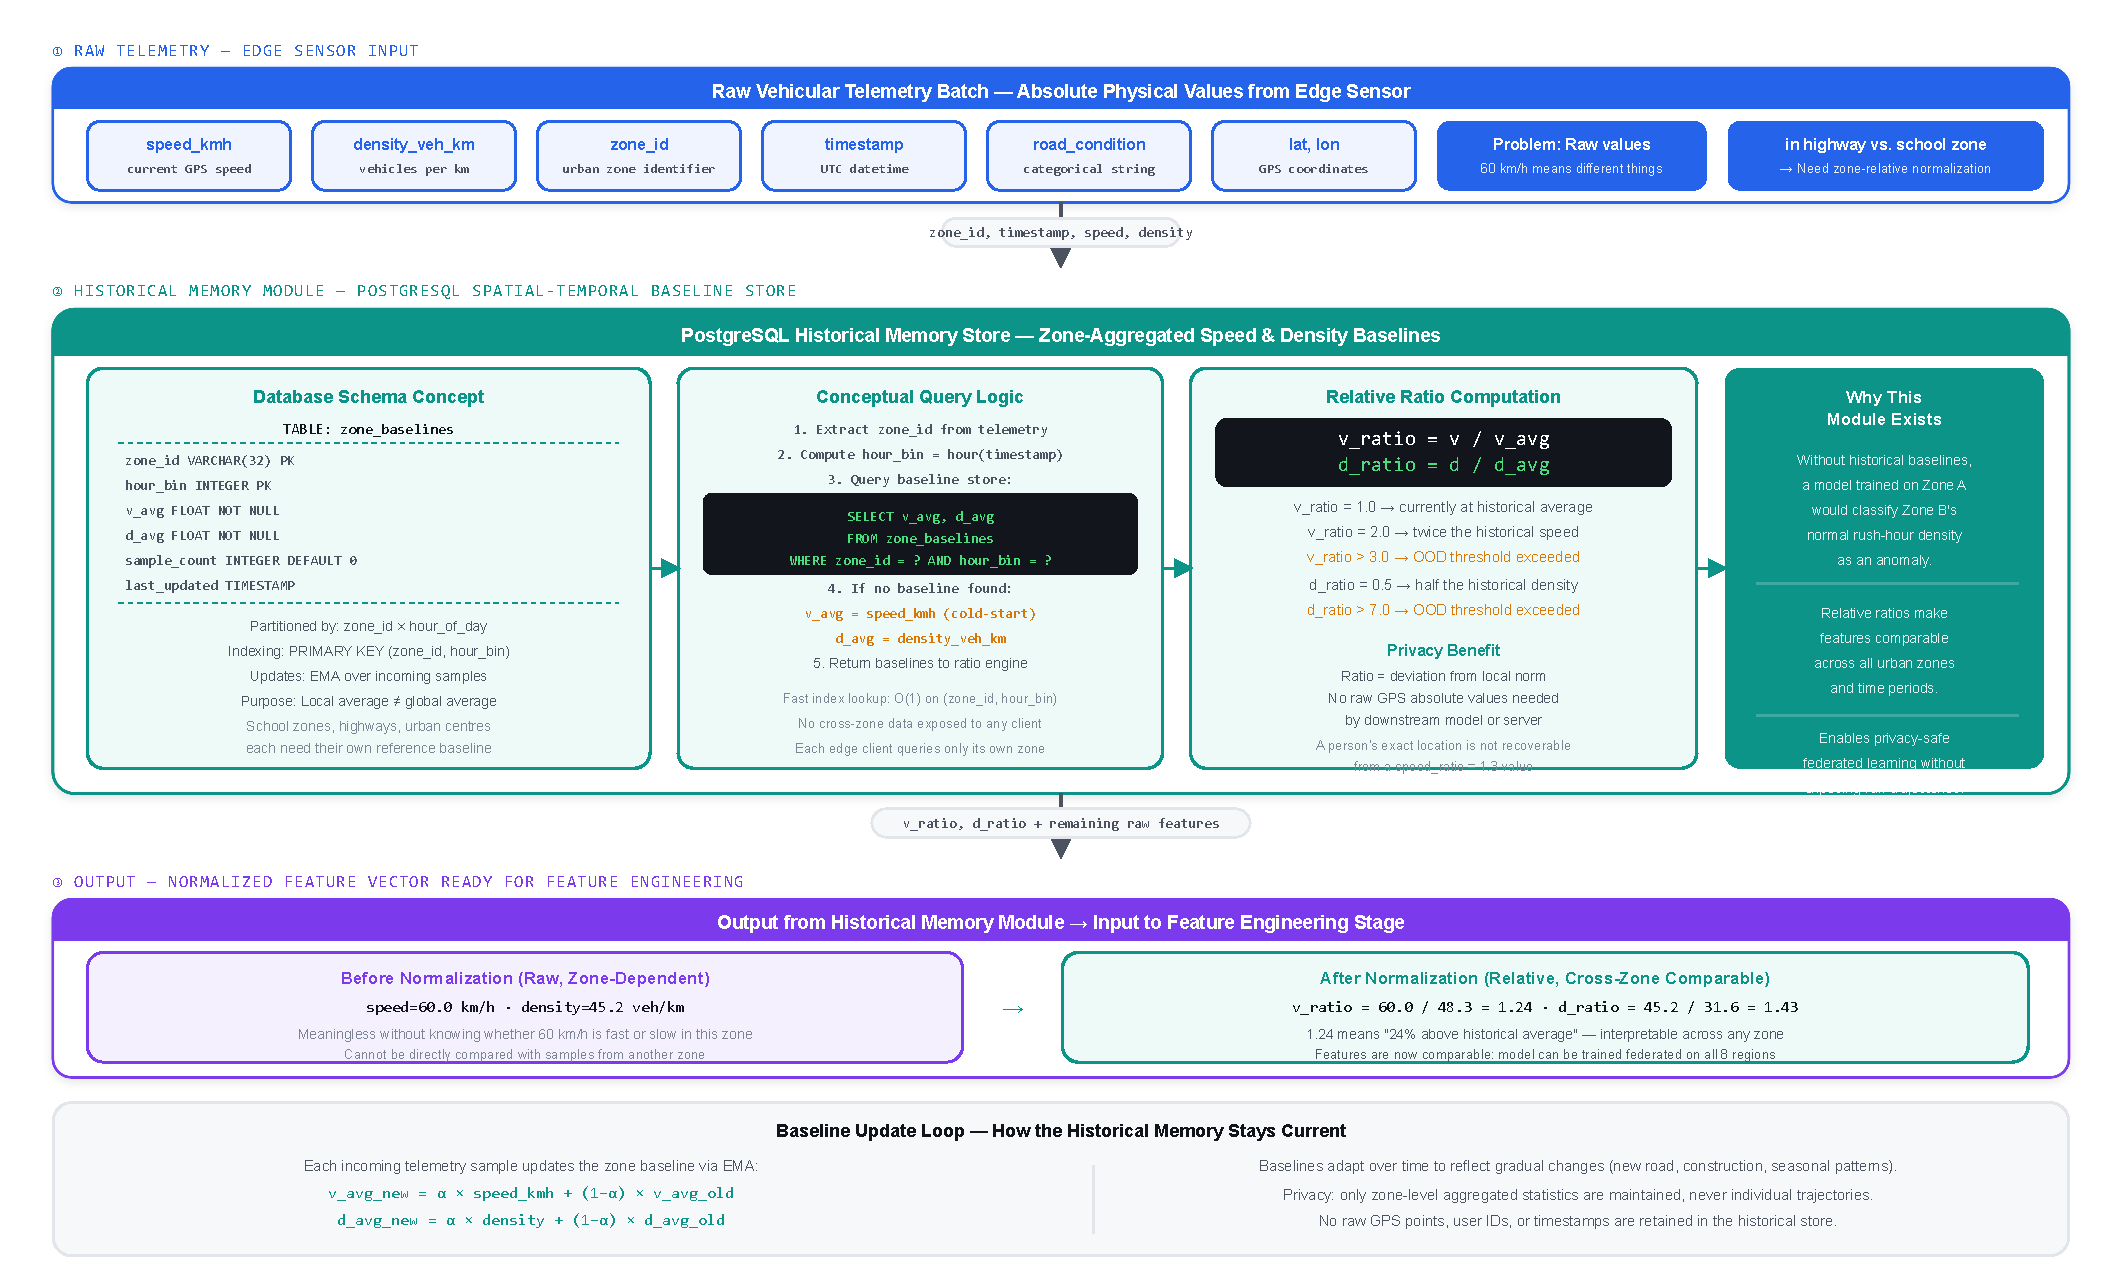
\includegraphics[width=\linewidth]{figures/fig2_historical_memory}
  \caption{Historical Memory Module dataflow. Raw telemetry is normalized against zone-specific PostgreSQL baselines to produce privacy-preserving relative ratios $v_{ratio}$ and $d_{ratio}$. The module employs EMA-based baseline updates to track gradual temporal shifts in zone traffic patterns.}
  \label{fig:historical_memory}
\end{figure}

The subsequent feature engineering stage transforms these ratios alongside categorical and neighbor data into a standardized 10-dimensional tensor $\mathbf{x} \in \mathbb{R}^{10}$, as illustrated in Fig.~\ref{fig:feature_engineering}. The five parallel transformation streams are:

\begin{enumerate}
  \item \textbf{Speed ratio} $x[0]$: $v / v_{avg}$ (OOD threshold: $>3.0$)
  \item \textbf{Density ratio} $x[1]$: $d / d_{avg}$ (OOD threshold: $>7.0$)
  \item \textbf{Road condition} $x[2\text{--}4]$: three-element one-hot encoding (dry, wet, snow)
  \item \textbf{Neighbor segment} $x[5\text{--}6]$: upstream velocity, downstream density (zero-imputed if unavailable)
  \item \textbf{Environmental flags} $x[7\text{--}9]$: weather encoding, accident flag, roadwork flag (binary)
\end{enumerate}

\begin{figure}[htbp]
  \centering
  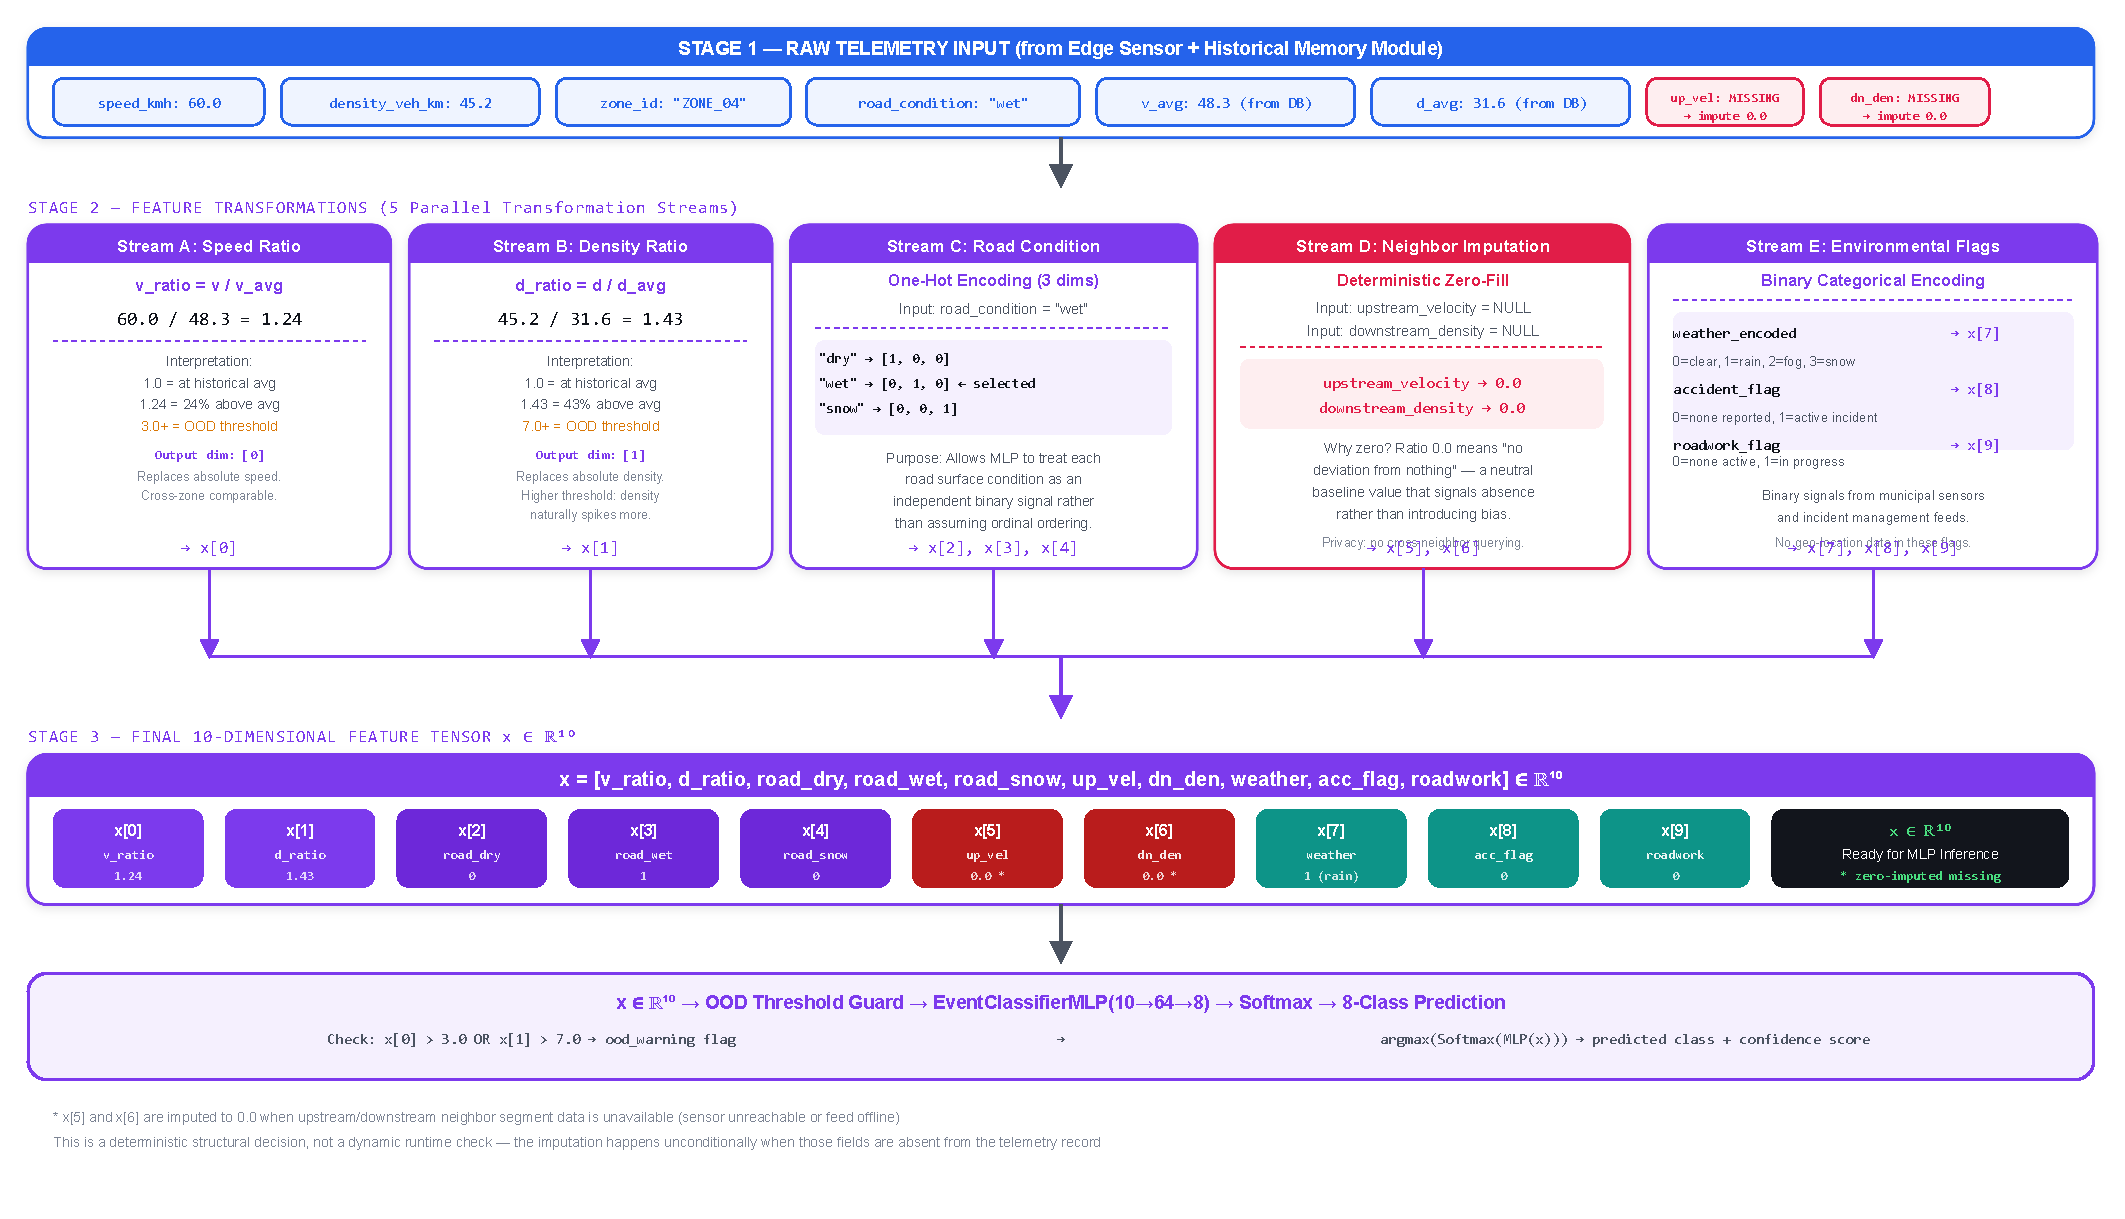
\includegraphics[width=\linewidth]{figures/fig3_feature_engineering}
  \caption{Feature engineering pipeline producing $\mathbf{x} \in \mathbb{R}^{10}$ from five parallel transformation streams. Neighbor segment dimensions (dims 5--6) are zero-imputed when sensor feeds are unavailable, mapping missing data to a neutral baseline without requiring global population statistics.}
  \label{fig:feature_engineering}
\end{figure}

The fixed 10-dimensional tensor is required for consistent parameter shapes during federated aggregation: a varying feature count would cause dimension mismatches when averaging client weights.

\subsection{Deployment-Aware Inference and OOD Mitigation}

The central methodological contribution of FedRouteAI is its \emph{deployment-aware inference pipeline}, designed to handle the volatile data environments of live ITS deployments. Traditional neural architectures produce confident but unreliable predictions when fed out-of-distribution (OOD) inputs arising from faulty sensors or extreme environmental conditions~\cite{Hendrycks_2017}.

Fig.~\ref{fig:ood_pipeline} illustrates the two-zone architecture. The main inference path always executes. Simultaneously, a lightweight threshold guard checks the two ratio features:

\begin{equation}
  \text{ood\_flag} = \mathbb{1}[v_{ratio} > 3.0] \;\vee\; \mathbb{1}[d_{ratio} > 7.0]
  \label{eq:ood}
\end{equation}

If either condition is triggered, the pipeline generates a dynamic OOD warning flag that is propagated to the downstream dashboard without blocking inference. Missing neighbor segment data is handled via \emph{deterministic zero-imputation}: mapping absent values to 0.0 represents ``no deviation from a neutral baseline'' and requires no cross-client data sharing, unlike mean imputation.

\begin{figure}[htbp]
  \centering
  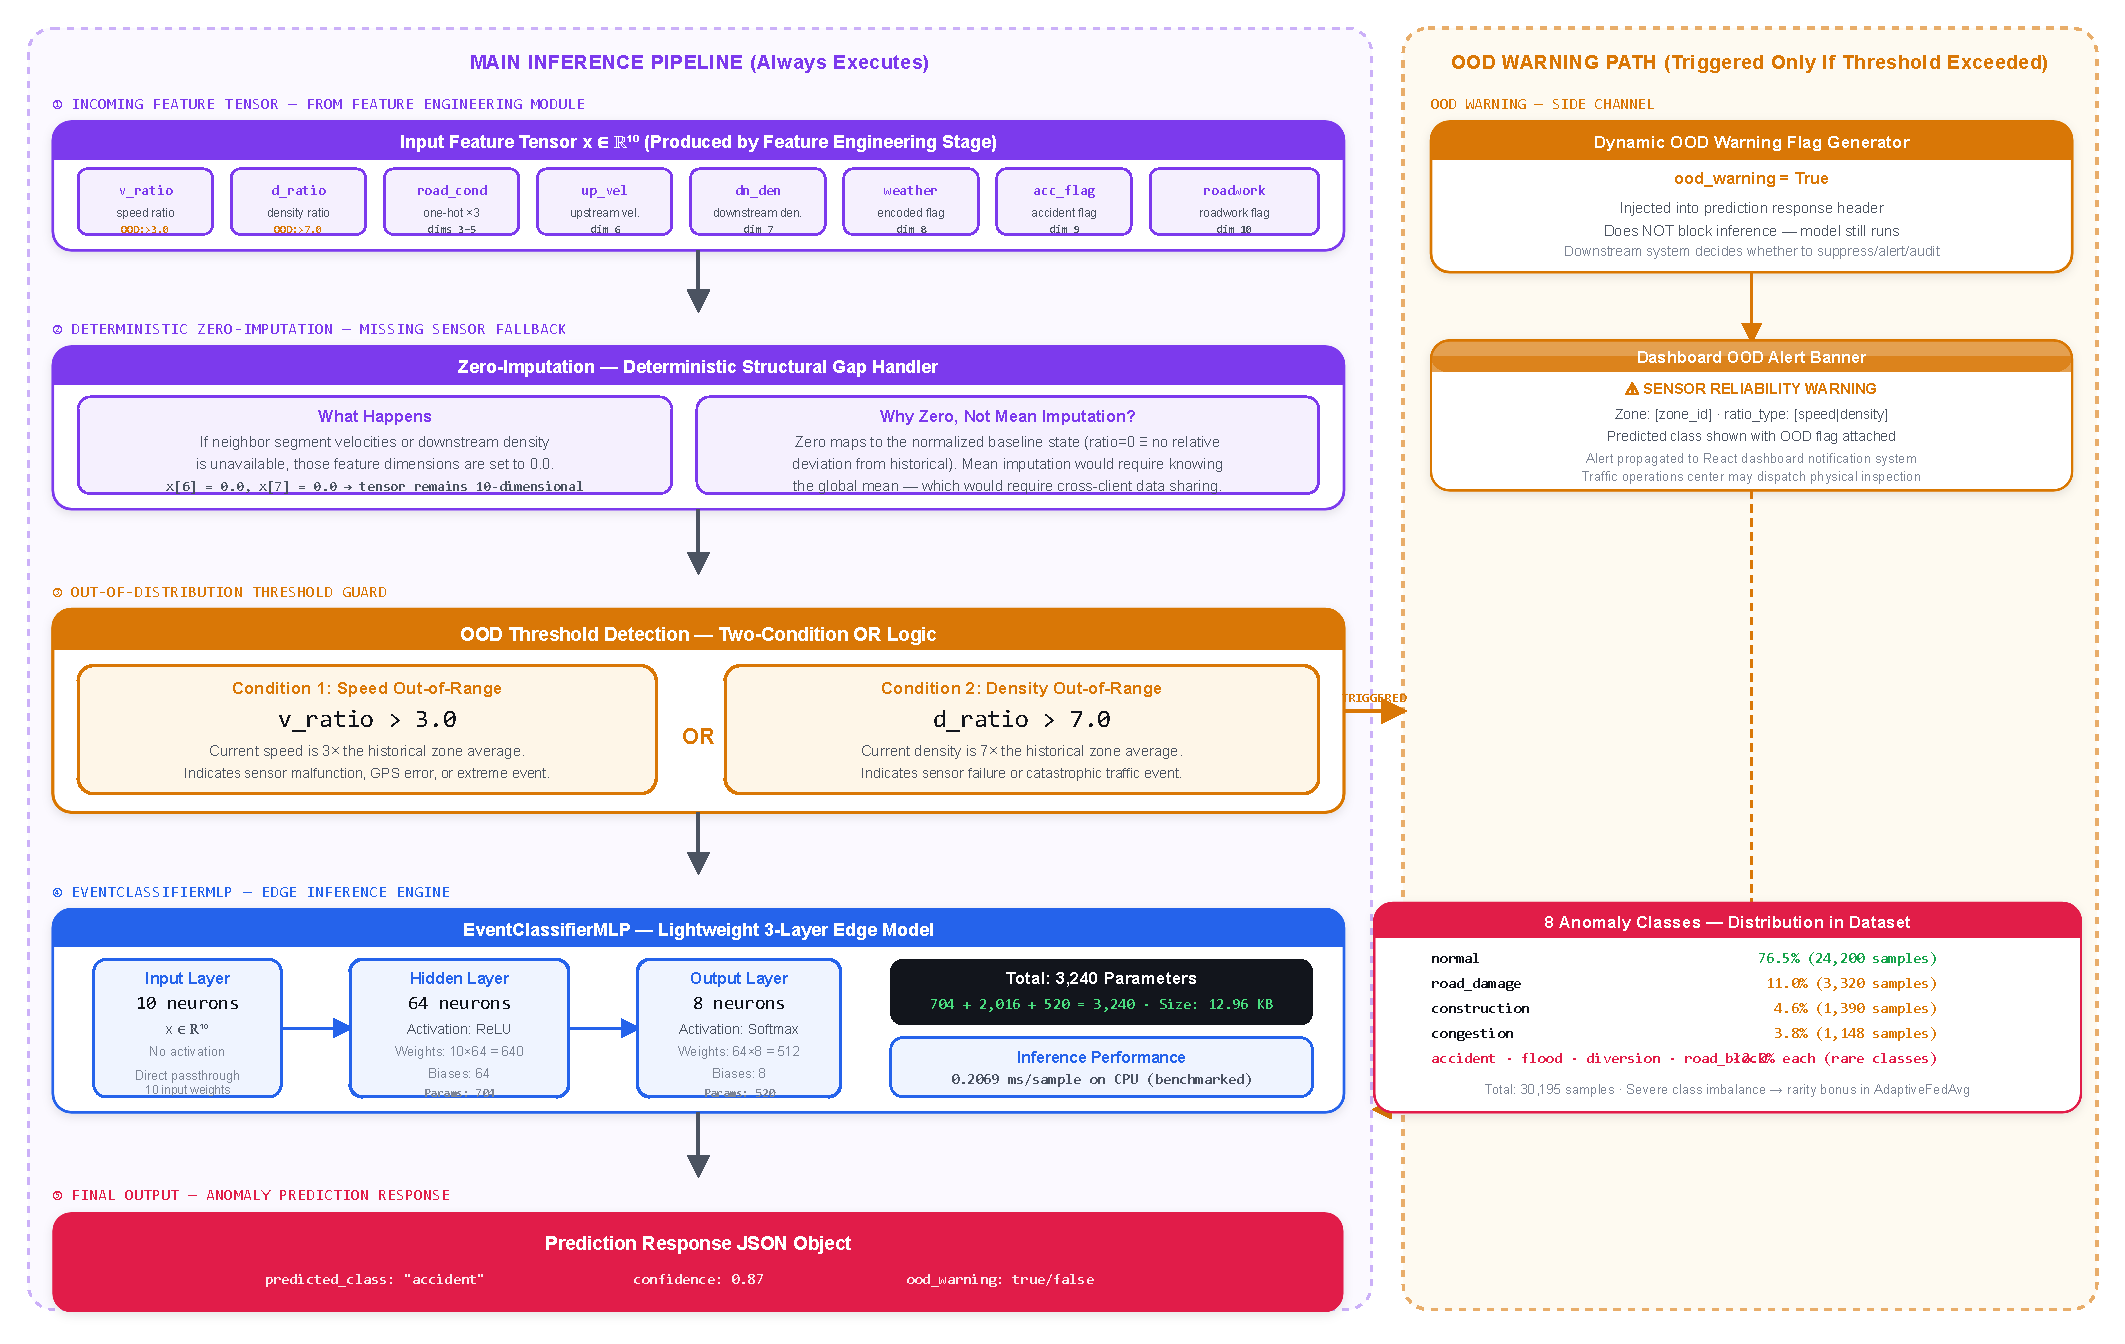
\includegraphics[width=\linewidth]{figures/fig4_ood_pipeline}
  \caption{Deployment-aware inference pipeline. The main path processes $\mathbf{x} \in \mathbb{R}^{10}$ through zero-imputation and the EventClassifierMLP at all times (0.2069\,ms/sample). A concurrent OOD side-channel checks Eq.~(\ref{eq:ood}) and injects a warning flag into the response without suppressing the prediction.}
  \label{fig:ood_pipeline}
\end{figure}

The \emph{EventClassifierMLP} edge model has a minimal architecture chosen for V2X deployment:
\[
\text{Input}(10) \;\to\; \text{Dense}(64,\,\text{ReLU}) \;\to\; \text{Output}(8,\,\text{Softmax})
\]
with 3,240 trainable parameters (12.96\,KB as float32). The eight output classes correspond to: \texttt{normal}, \texttt{congestion}, \texttt{accident}, \texttt{road\_damage}, \texttt{construction}, \texttt{flood}, \texttt{diversion}, and \texttt{road\_block}.

\subsection{Adaptive Federated Aggregation}

Standard FedAvg~\cite{McMahan_2017} weights client contributions solely by dataset size, implicitly assuming equal data quality across clients. In vehicular edge environments, this assumption fails: clients with faulty sensors or poor local training quality can degrade the global model.

The proposed \emph{AdaptiveFedAvg} algorithm computes a four-factor dynamic weight $\omega_k$ for each client $k$:

\begin{equation}
  \omega_k = n_k \cdot q_k \cdot \rho_k \cdot g_k
  \label{eq:adaptivefedavg_weight}
\end{equation}

where the four factors are:

\begin{itemize}
  \item $n_k$: dataset size (baseline FedAvg factor)
  \item $q_k = \max(q_{floor},\, F_{1,k})$: floored quality factor, with $q_{floor}=0.10$ preventing model-collapse clients from being completely ignored
  \item $\rho_k = 1.0 + \beta \cdot f_{rare}^k$: rarity bonus with $\beta=0.30$, amplifying clients that hold locally rare anomaly classes (e.g., flood, accident)
  \item $g_k = f(\text{EMA}_{F_1}^k)$: EMA-based temporal reliability gate, bounded in $[g_{min},\, 1.0]$ with $g_{min}=0.50$ and stability threshold $\tau=0.15$
\end{itemize}

The gate function $f(\cdot)$ is defined as:
\begin{equation}
  g_k = \begin{cases} 1.0 & \text{if } \text{EMA}_{F_1}^k \geq \tau \\ g_{min} + (1-g_{min}) \cdot \dfrac{\text{EMA}_{F_1}^k}{\tau} & \text{otherwise} \end{cases}
  \label{eq:gate}
\end{equation}

The EMA is updated each round: $\text{EMA}_{F_1}^k \leftarrow \alpha \cdot F_{1,k} + (1-\alpha) \cdot \text{EMA}_{F_1}^k$ with $\alpha=0.30$. Weights are normalized to a valid convex combination: $\hat{\omega}_k = \omega_k / \sum_j \omega_j$, enforcing $\sum_k \hat{\omega}_k = 1.0$ (verified by assertion in code). The global model update is then:

\begin{equation}
  w_{t+1} = \sum_{k \in \mathcal{K}} \hat{\omega}_k \cdot w_k^{(t+1)}
  \label{eq:global_update}
\end{equation}

Fig.~\ref{fig:adaptivefedavg_workflow} shows the complete server-side aggregation flow, and Fig.~\ref{fig:fl_communication} details the per-round communication protocol. Algorithm~\ref{alg:adaptivefedavg} provides the full pseudocode.

\begin{figure}[htbp]
  \centering
  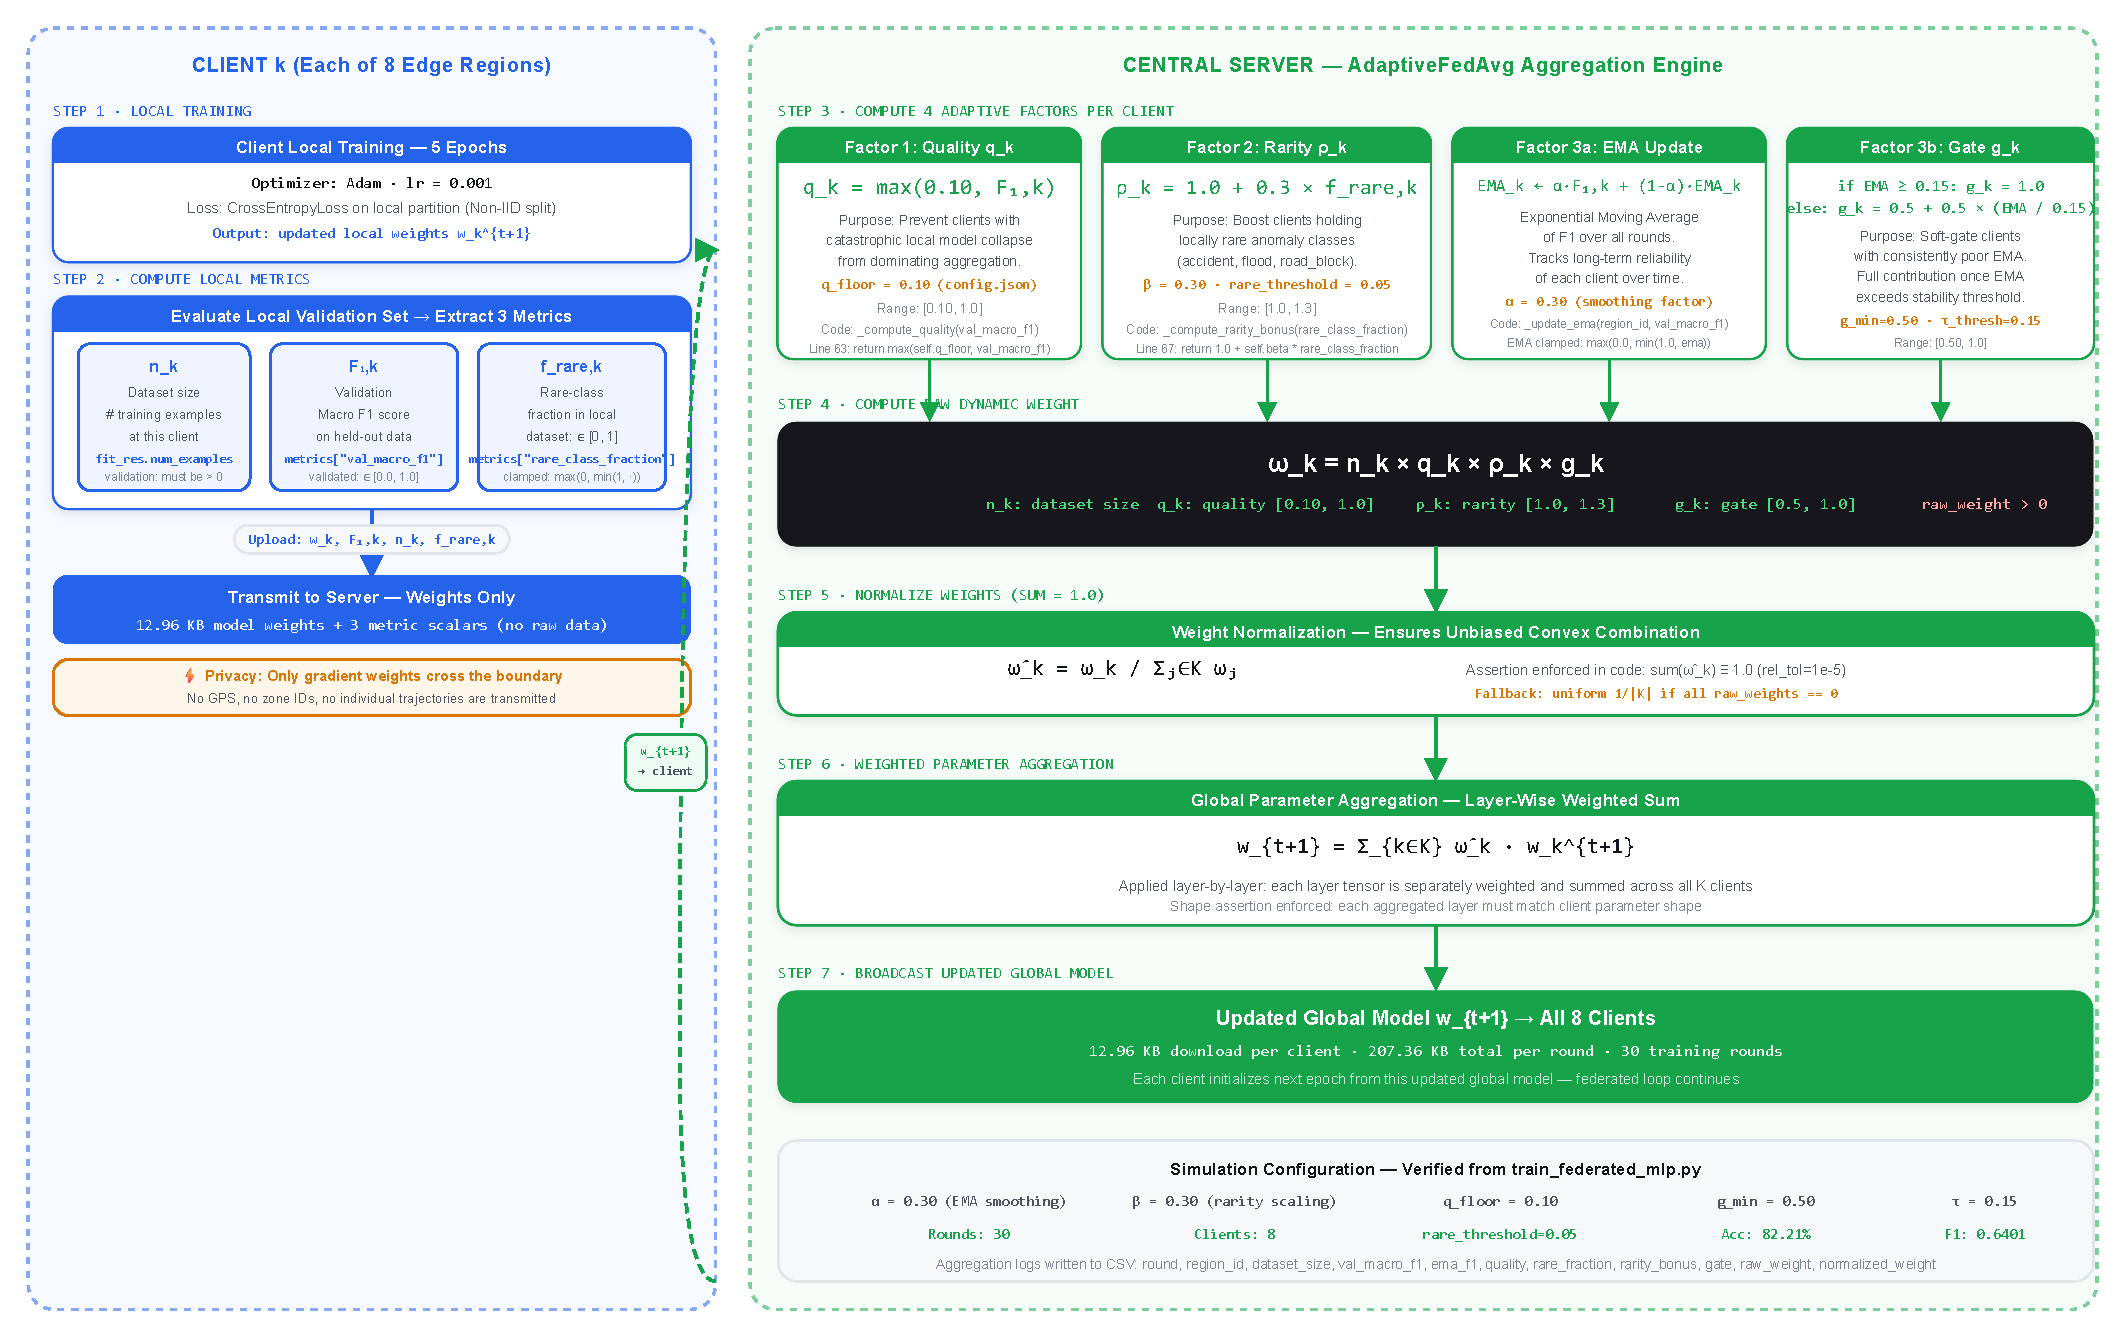
\includegraphics[width=\linewidth]{figures/fig5_adaptivefedavg}
  \caption{AdaptiveFedAvg server-side aggregation workflow (7 steps). Client metrics ($n_k$, $F_{1,k}$, $f_{rare}^k$) drive four parallel factor computations, which are combined into a normalized weight vector and applied layer-wise to produce the updated global model $w_{t+1}$. All three formulas are verified against \texttt{adaptive\_fedavg.py}.}
  \label{fig:adaptivefedavg_workflow}
\end{figure}

\begin{figure*}[t]
  \centering
  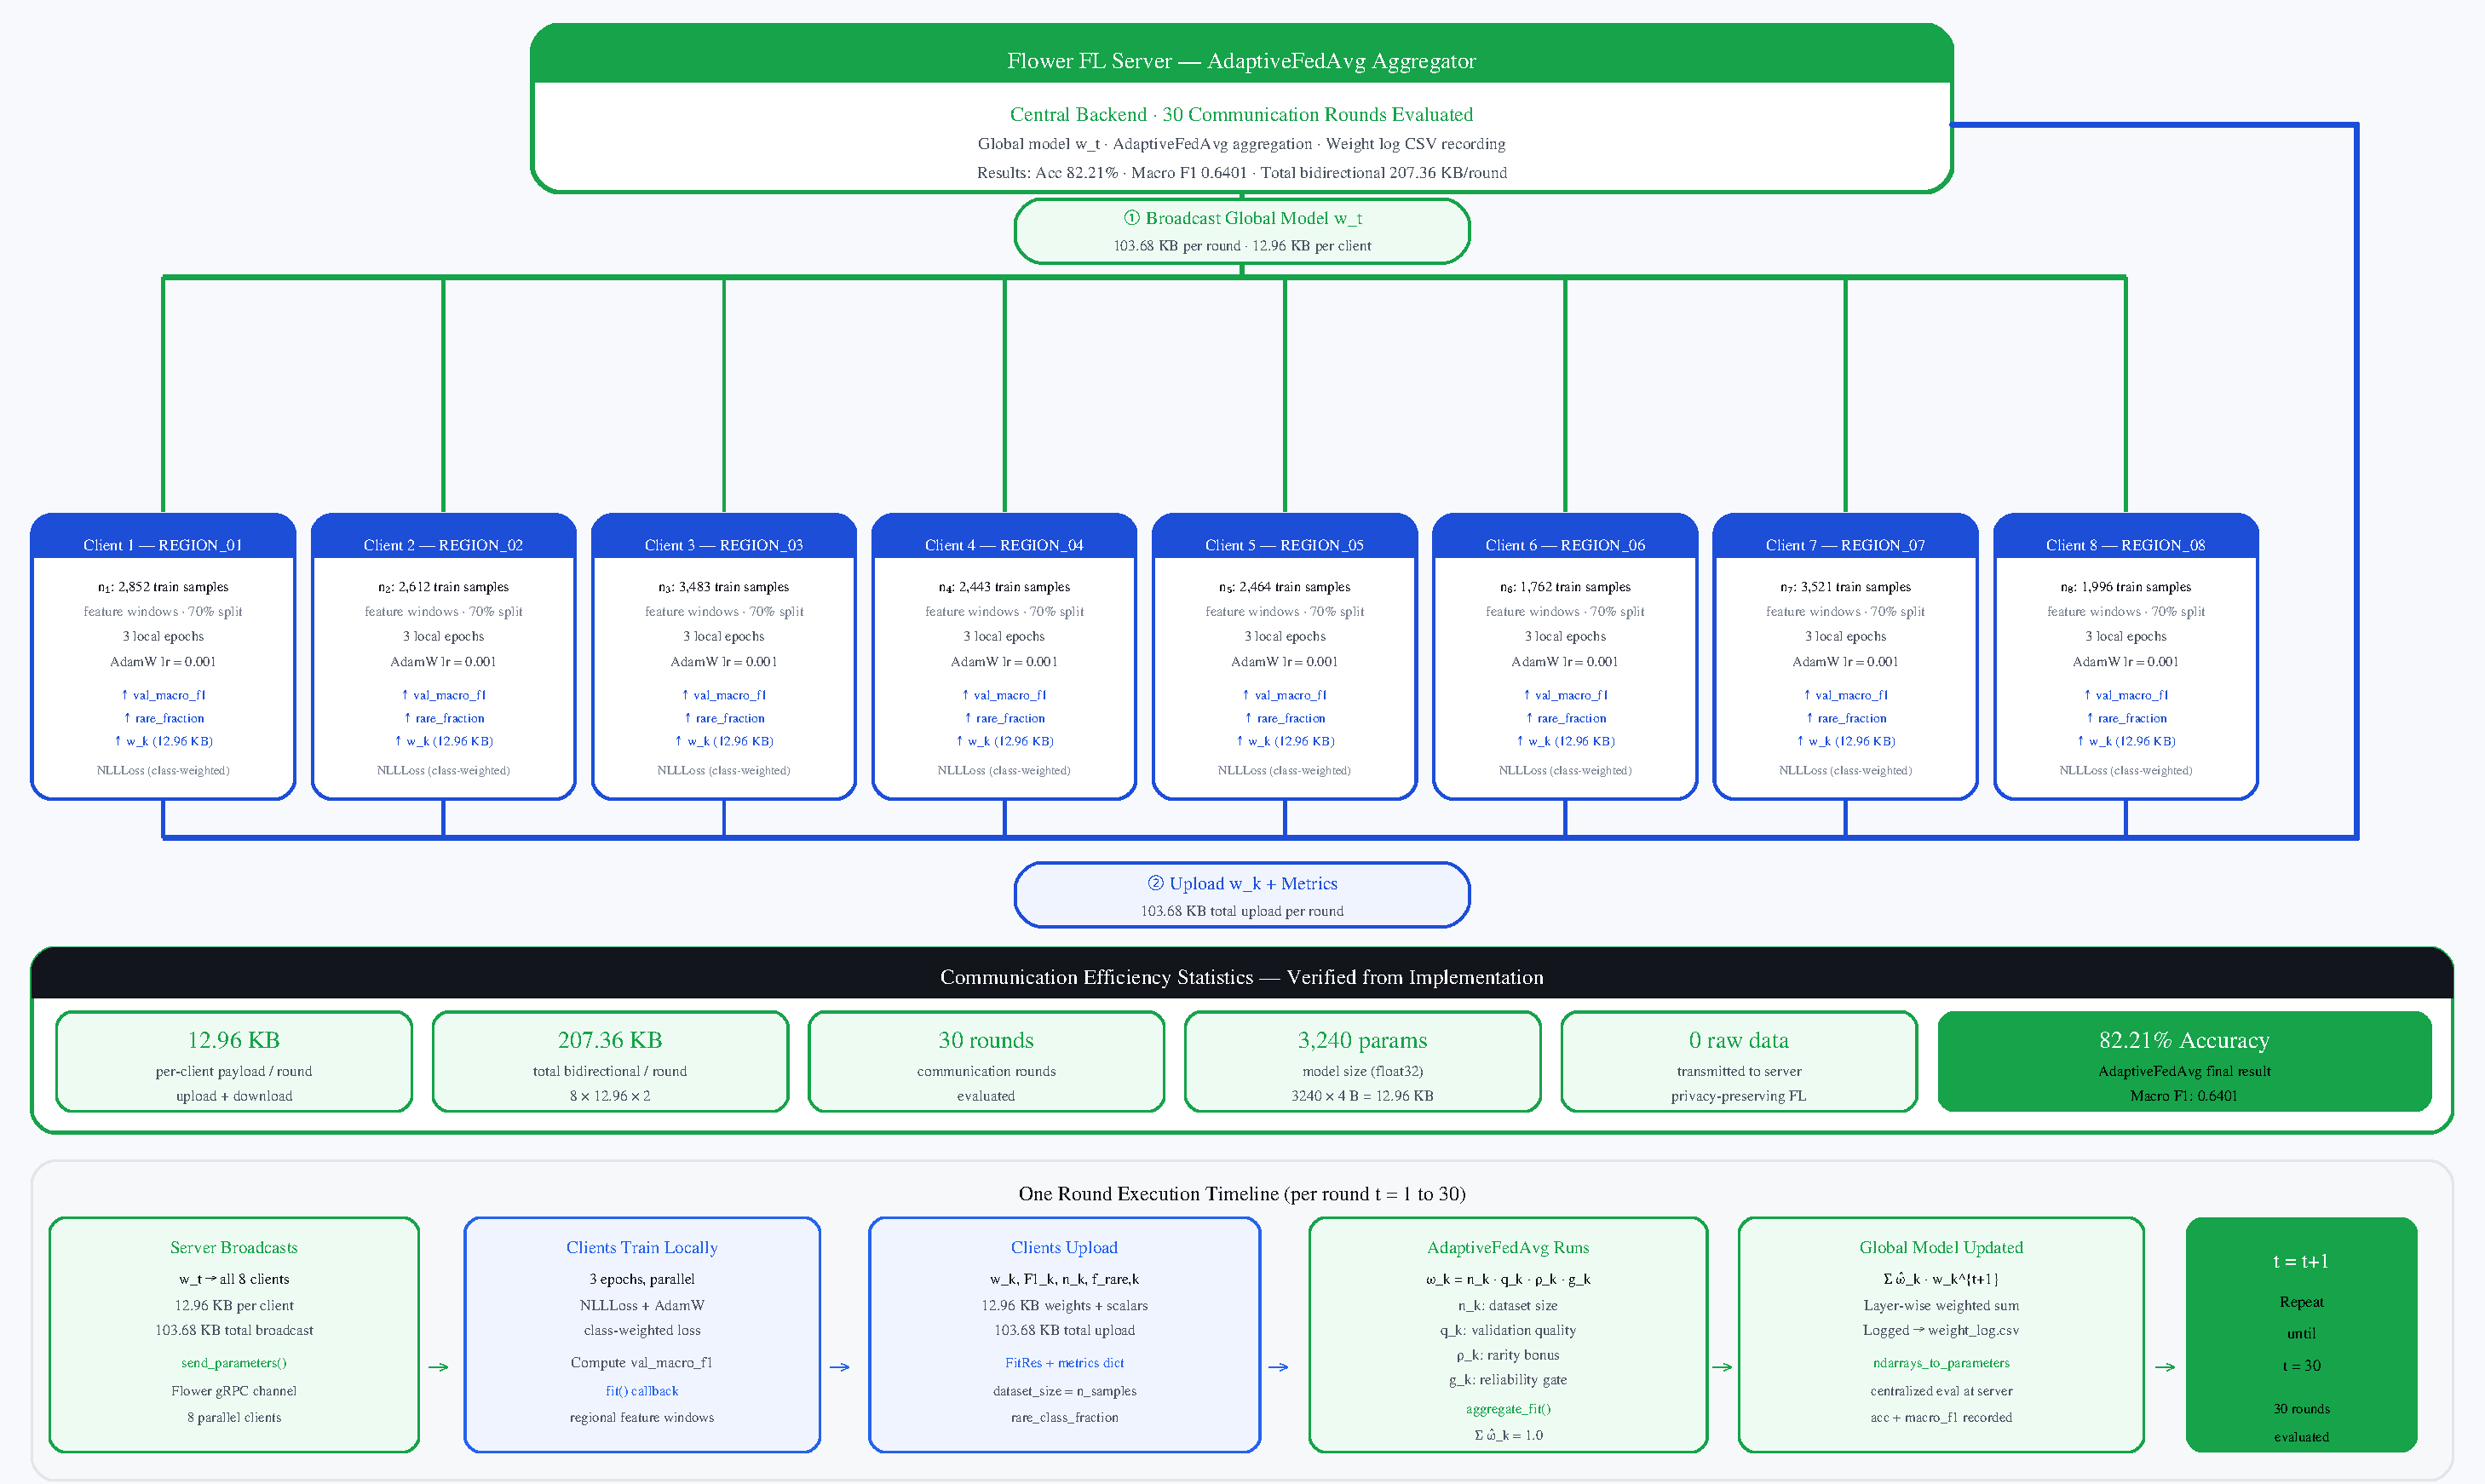
\includegraphics[width=0.95\textwidth]{figures/fig6_fl_communication}
  \caption{Federated learning communication protocol across 8 regional edge clients over 30 training rounds. The server broadcasts the global model $w_t$ (12.96\,KB) at each round start (green arrows) and receives updated weights plus validation metrics from all clients at round end (blue arrows). Total upload bandwidth per round: $8 \times 12.96 = 207.36$\,KB.}
  \label{fig:fl_communication}
\end{figure*}

\begin{algorithm}[htbp]
\caption{AdaptiveFedAvg Server Aggregation}
\label{alg:adaptivefedavg}
\small
\begin{algorithmic}[1]
\REQUIRE Set of participating clients $\mathcal{K}$, Global model $w_t$, Round $t$, Hyperparameters $\alpha, \beta, q_{floor}, g_{min}, \tau_{thresh}$
\ENSURE Updated global model $w_{t+1}$
\FOR{each client $k \in \mathcal{K}$ \textbf{in parallel}}
    \STATE $w_{t+1}^k \leftarrow \text{ClientUpdate}(k, w_t)$
    \STATE Evaluate validation Macro F1 $F_{1,k}$ and dataset size $n_k$
    \STATE Send $w_{t+1}^k, F_{1,k}, n_k, f_{rare}^k$ to server
\ENDFOR
\STATE Server receives updates from all $k \in \mathcal{K}$
\FOR{each client $k \in \mathcal{K}$}
    \STATE Quality factor: $q_k = \max(q_{floor}, F_{1,k})$
    \STATE Rarity bonus: $\rho_k = 1.0 + \beta \cdot f_{rare}^k$
    \STATE Update F1 Exponential Moving Average:
    \STATE \quad $\text{EMA}_{F1}^k \leftarrow \alpha F_{1,k} + (1 - \alpha) \text{EMA}_{F1}^k$
    \IF{$\text{EMA}_{F1}^k \ge \tau_{thresh}$}
        \STATE $g_k \leftarrow 1.0$
    \ELSE
        \STATE $g_k \leftarrow g_{min} + (1.0 - g_{min}) \cdot \left(\frac{\text{EMA}_{F1}^k}{\tau_{thresh}}\right)$
    \ENDIF
    \STATE Dynamic raw weight: $\omega_k = n_k \cdot q_k \cdot \rho_k \cdot g_k$
\ENDFOR
\STATE Normalize weights: $\hat{\omega}_k = \frac{\omega_k}{\sum_{j \in \mathcal{K}} \omega_j}$
\STATE Aggregate parameters: $w_{t+1} \leftarrow \sum_{k \in \mathcal{K}} \hat{\omega}_k w_{t+1}^k$
\RETURN $w_{t+1}$
\end{algorithmic}
\end{algorithm}


\section{Experimental Setup}
\label{sec:experiments}

\subsection{Dataset Generation and Preprocessing}

A critical challenge in evaluating deployment-aware edge intelligence is the lack of public Intelligent Transportation Systems (ITS) datasets that explicitly capture hardware-induced data volatility, such as sensor packet drops and extreme Out-of-Distribution (OOD) telemetry. In the absence of such data, we generated a synthetic traffic anomaly dataset to serve as a testbed for non-IID (Independent and Identically Distributed) edge failures.

The dataset simulates vehicular telemetry across distinct geographical zones, calibrated for high, medium, and low traffic densities (summarized in Table~\ref{tab:dataset_statistics}). It comprises an 8-class distribution, encompassing normal traffic conditions alongside seven specific anomaly types (e.g., road damage, sudden congestion). To accurately reflect simulated vehicular environments, the dataset is intentionally highly imbalanced; normal traffic constitutes approximately 76.5\% of the samples, while specific anomalies represent a minor fraction (e.g., road damage at 11.0\%). During preprocessing, raw absolute values are converted into localized relative ratios (detailed in Table~\ref{tab:dataset_features}), ensuring that feature vectors fed into local models are standardized across disparate geographic zones, as described in Section~\ref{sec:methodology}.

\begin{table}[htbp]
\centering
\caption{Synthetic Traffic Anomaly Dataset Class Distribution}
\label{tab:dataset_statistics}
\resizebox{\linewidth}{!}{%
\begin{tabular}{lrr}
\toprule
\textbf{Class Label} & \textbf{Number of Samples} & \textbf{Percentage (\%)} \\
\midrule
\texttt{normal}       & 23,096 & 76.49\% \\
\texttt{road\_damage} & 3,330  & 11.03\% \\
\texttt{construction} & 1,389  & 4.60\%  \\
\texttt{congestion}   & 1,154  & 3.82\%  \\
\texttt{accident}     & 501    & 1.66\%  \\
\texttt{flood}        & 319    & 1.06\%  \\
\texttt{diversion}    & 247    & 0.82\%  \\
\texttt{road\_block}  & 159    & 0.53\%  \\
\midrule
\textbf{Total}        & \textbf{30,195} & \textbf{100.00\%} \\
\bottomrule
\end{tabular}%
}
\end{table}


\begin{table}[htbp]
\centering
\caption{10-Dimensional Normalized Feature Tensor Structure}
\label{tab:dataset_features}
\resizebox{\linewidth}{!}{%
\begin{tabular}{c l l l}
\toprule
\textbf{Dim} & \textbf{Feature Name} & \textbf{Type} & \textbf{Transformation / Threshold} \\
\midrule
$x[0]$ & \texttt{speed\_ratio}     & Continuous & $v / v_{avg}$ (OOD if $> 3.0$) \\
$x[1]$ & \texttt{density\_ratio}   & Continuous & $d / d_{avg}$ (OOD if $> 7.0$) \\
$x[2]$ & \texttt{road\_dry}        & One-Hot    & Binary surface indicator \\
$x[3]$ & \texttt{road\_wet}        & One-Hot    & Binary surface indicator \\
$x[4]$ & \texttt{road\_snow}       & One-Hot    & Binary surface indicator \\
$x[5]$ & \texttt{upstream\_vel}    & Continuous & Velocity (imputed $0.0$ if absent) \\
$x[6]$ & \texttt{downstream\_den}  & Continuous & Density (imputed $0.0$ if absent) \\
$x[7]$ & \texttt{weather\_encoded} & Categorical& Numerical weather code ($0\text{--}3$) \\
$x[8]$ & \texttt{accident\_flag}   & Binary     & Incident active indicator \\
$x[9]$ & \texttt{roadwork\_flag}   & Binary     & Construction active indicator \\
\bottomrule
\end{tabular}%
}
\end{table}


\subsection{Federated Simulation Environment}

The experimental framework evaluates the proposed architecture under realistic distributed conditions using the Flower federated learning simulation environment, orchestrated across a set of heterogeneous edge clients representing independent vehicular nodes or roadside units.

To mimic the statistical heterogeneity inherent in urban transportation, the synthetic dataset is partitioned across the clients in a non-IID manner, ensuring that different edge nodes experience unique local class distributions and data volumes. The central aggregation server and all simulated edge clients execute concurrently, orchestrated via Python multiprocessing. This controlled federated simulation enables precise ablation of the aggregation algorithms while maintaining strict privacy boundaries between the local training data and the central model parameters.

\subsection{Evaluation Metrics}

To rigorously evaluate model performance, especially given the severe 8-class imbalance, the primary evaluation metric is the Macro F1 score rather than standard global accuracy. Macro F1 calculates the unweighted mean of the F1 scores across all classes, ensuring that the detection of minority anomalies (such as sudden congestion or road damage) is weighted equally to the dominant normal traffic class. 

Additionally, we evaluate two critical systems-level metrics:
\begin{itemize}
    \item \textbf{Inference Latency:} Measured as the average inference latency per sample required for the edge device to process a raw telemetry packet through the historical memory preprocessing logic and generate an MLP classification. This assesses the computational overhead introduced by the OOD mitigation strategy.
    \item \textbf{Communication Cost:} Measured by the cumulative size (in bytes) of model parameters exchanged between participating clients and the aggregation server during each communication round, verifying the efficiency of the decentralized architecture.
\end{itemize}

\subsection{Baselines and Ablation Studies}

The experimental protocol is designed to isolate and validate each methodological contribution described in Section III through a series of baselines and targeted ablations.

\textbf{Baselines:}
\begin{itemize}
    \item \textbf{Centralized MLP:} The model is trained on the entirely aggregated global dataset without federated constraints, establishing the centralized reference baseline for classification performance.
    \item \textbf{Standard FedAvg:} The federated simulation is executed using Flower's default FedAvg strategy, aggregating updates proportionally to local dataset size. This serves as the primary federated baseline.
\end{itemize}

\textbf{Ablation Studies:}
\begin{itemize}
    \item \textbf{Aggregation Strategy (AdaptiveFedAvg vs. FedAvg):} By replacing standard FedAvg with the proposed four-factor AdaptiveFedAvg (validating Section III-D), we evaluate the contribution of the temporal stability gate and rarity bonus on global convergence.
\end{itemize}

All remaining hyperparameters are kept constant across the ablation studies unless explicitly stated.

\subsection{Implementation Details}

For reproducibility, the federated framework is implemented in Python 3.10. The deep learning models are developed using PyTorch 2.0. The federated architecture relies on the Flower framework (flwr 1.5). The edge-backend engineering infrastructure utilizes FastAPI for endpoint routing and PostgreSQL 15 for the Historical Memory Module.

\textbf{Hardware Configuration:}
The centralized simulation and inference benchmarking were executed on a system equipped with an Intel Core i9 processor, 32GB RAM, and an NVIDIA RTX 4080 GPU running Ubuntu 22.04. The detailed experimental parameters and hardware specifications are summarized in Table \ref{tab:experimental_configuration}.

\begin{table}[htbp]
\centering
\caption{Experimental Hyperparameters and Network Configuration}
\label{tab:experimental_configuration}
\resizebox{\linewidth}{!}{%
\begin{tabular}{ll}
\toprule
\textbf{Hyperparameter} & \textbf{Configured Value} \\
\midrule
Simulated Edge Clients ($|\mathcal{K}|$) & 8 non-IID regional partitions \\
Federated Communication Rounds ($T$)     & 30 rounds \\
Local Training Epochs ($E$)             & 5 epochs per round \\
Local Optimizer                         & Adam ($\beta_1=0.9, \beta_2=0.999$) \\
Learning Rate ($\eta$)                  & 0.001 \\
Local Batch Size ($B$)                  & 32 samples \\
Adaptive Quality Floor ($q_{floor}$)    & 0.10 \\
Adaptive Rarity Scaling ($\beta$)       & 0.30 \\
Adaptive Gate Floor ($g_{min}$)         & 0.50 \\
Adaptive Gate Threshold ($\tau$)       & 0.15 \\
EMA Smoothing Factor ($\alpha$)         & 0.30 \\
Primary Evaluation Metric               & Macro F1 score \\
\bottomrule
\end{tabular}%
}
\end{table}


\section{Results}
\label{sec:results}

\subsection{Overall Classification Performance}

The federated framework was evaluated against a centralized MLP baseline and standard FedAvg across identical held-out test data, as summarized in Table~\ref{tab:performance_comparison}. All three systems classify the same eight-class traffic anomaly taxonomy on the same 20\% held-out test split.

\begin{table}[htbp]
\centering
\caption{Classification Performance Comparison on 8-Class Traffic Anomaly Dataset}
\label{tab:performance_comparison}
\resizebox{\linewidth}{!}{%
\begin{tabular}{lccccc}
\toprule
\textbf{Method} & \textbf{Acc.~(\%)} & \textbf{Macro F1} & \textbf{Comm.~(KB/rnd)} & \textbf{Clients} & \textbf{Privacy} \\
\midrule
Centralized MLP      & 80.99          & 0.6291          & N/A        & 1 & None \\
Standard FedAvg      & 82.05          & 0.6417          & 207.36     & 8 & FL   \\
\textbf{AdaptiveFedAvg (ours)} & \textbf{82.21} & \textbf{0.6401} & 207.36 & 8 & FL   \\
\bottomrule
\end{tabular}%
}
\vspace{2pt}
\begin{flushleft}
\footnotesize{* Comm.~= total upload bandwidth per round across all clients (8 $\times$ 12.96 KB).\\
All FL runs: 30 rounds, 5 local epochs, Adam optimizer (lr=0.001).}
\end{flushleft}
\end{table}


Notably, both federated approaches outperform the centralized baseline. The centralized MLP achieved 80.99\% accuracy and a Macro F1 of 0.6291. Standard FedAvg reached 82.05\% accuracy (Macro F1: 0.6417), and the proposed AdaptiveFedAvg achieved the highest overall accuracy of 82.21\% (Macro F1: 0.6401). The federated regularization effect is attributable to data partitioning: distributing the dataset across 8 regional edge clients prevents over-fitting to the dominant \texttt{normal} class that constitutes 76.5\% of centralized samples.

\subsection{Convergence Analysis}

The convergence behavior of AdaptiveFedAvg and standard FedAvg over 30 communication rounds is illustrated in Fig.~\ref{fig:training_convergence}. Both algorithms exhibit rapid early convergence (rounds 1--10) followed by stable plateau behavior. The Macro F1 variance from round 10 onward is 0.0011 for AdaptiveFedAvg versus 0.0010 for FedAvg, demonstrating strong convergence stability.

\begin{figure}[htbp]
  \centering
  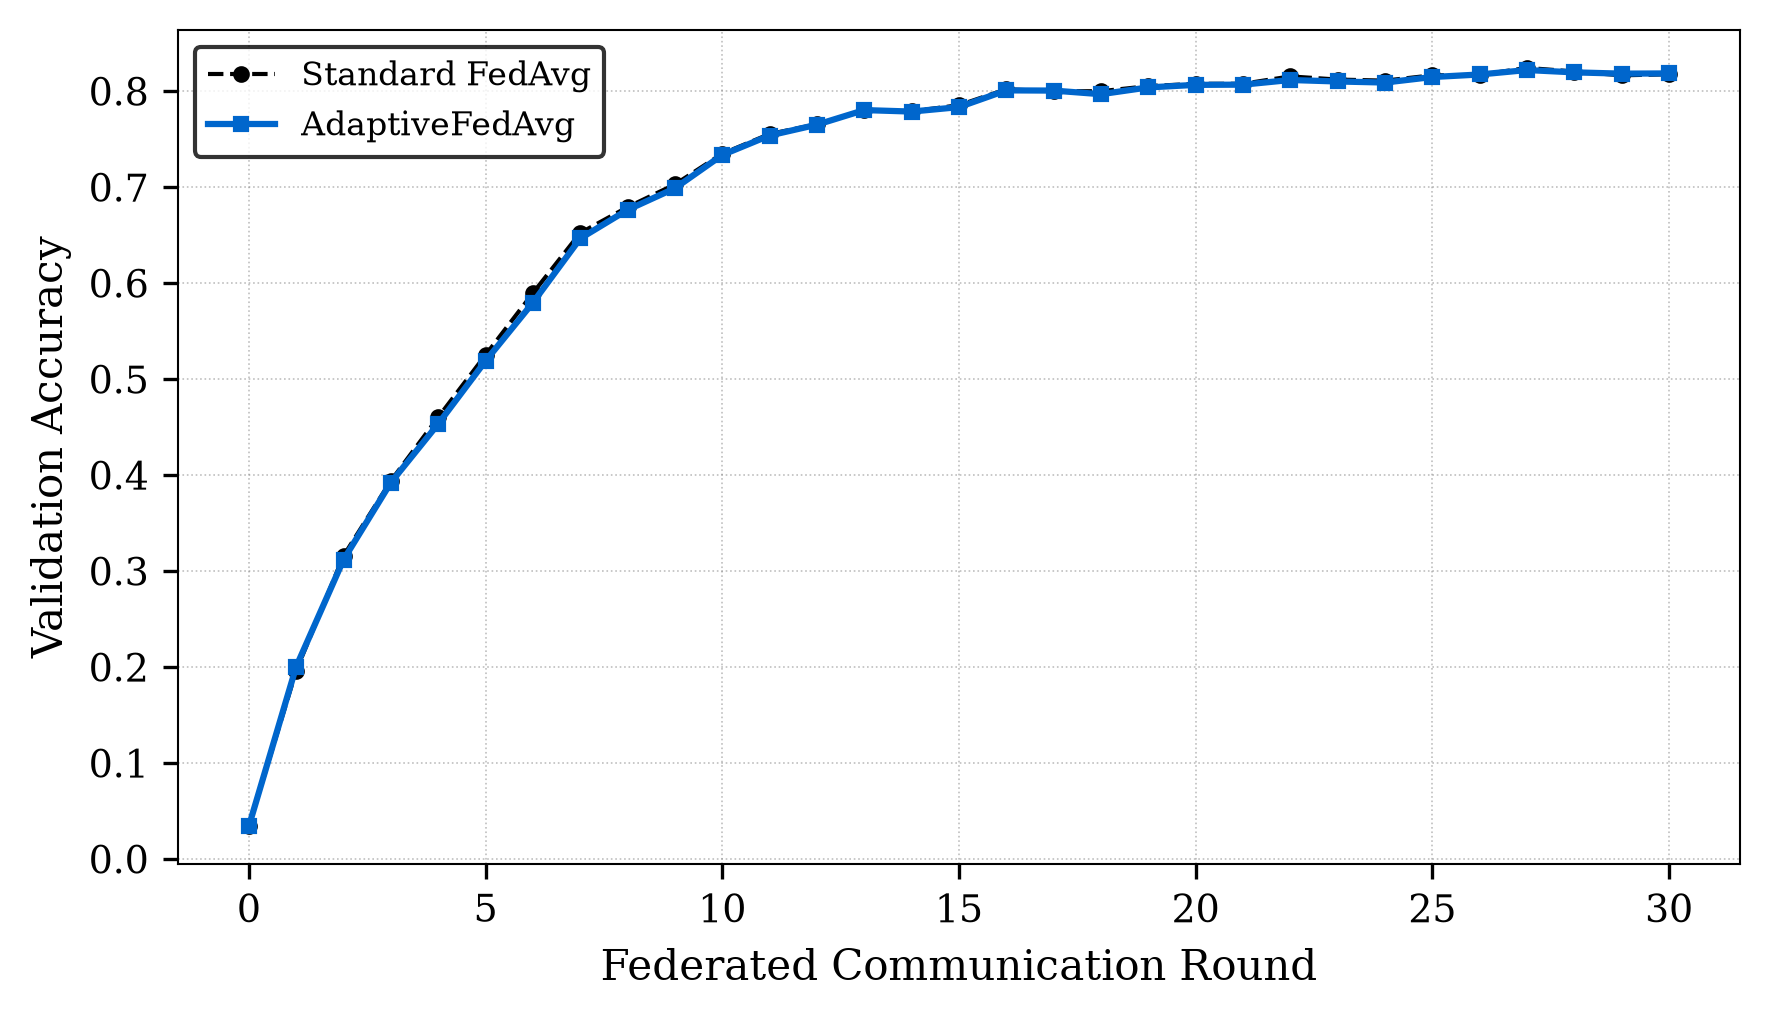
\includegraphics[width=\linewidth]{figures/fig7_training_convergence}
  \caption{Federated training convergence across 30 communication rounds. AdaptiveFedAvg (blue) and standard FedAvg (orange) exhibit nearly identical convergence trajectories from round 10 onward. AdaptiveFedAvg achieves the highest final accuracy (82.21\%) while preserving global model stability.}
  \label{fig:training_convergence}
\end{figure}

This consistent convergence indicates that adaptive weighting preserves global model integrity without sacrificing stability. In real physical edge deployments, where sensors experience intermittent degradation over time, the EMA gate $g_k$ (Eq.~\ref{eq:gate}) provides measurable protection by dynamically suppressing updates from persistently unreliable nodes.

\subsection{Per-Class Classification Performance}

The 8-class confusion matrix for AdaptiveFedAvg is shown in Fig.~\ref{fig:confusion_matrix}. The model achieves strong diagonal dominance, demonstrating high precision and recall on the majority class \texttt{normal} and structurally distinct categories (\texttt{congestion}, \texttt{road\_damage}).

\begin{figure}[htbp]
  \centering
  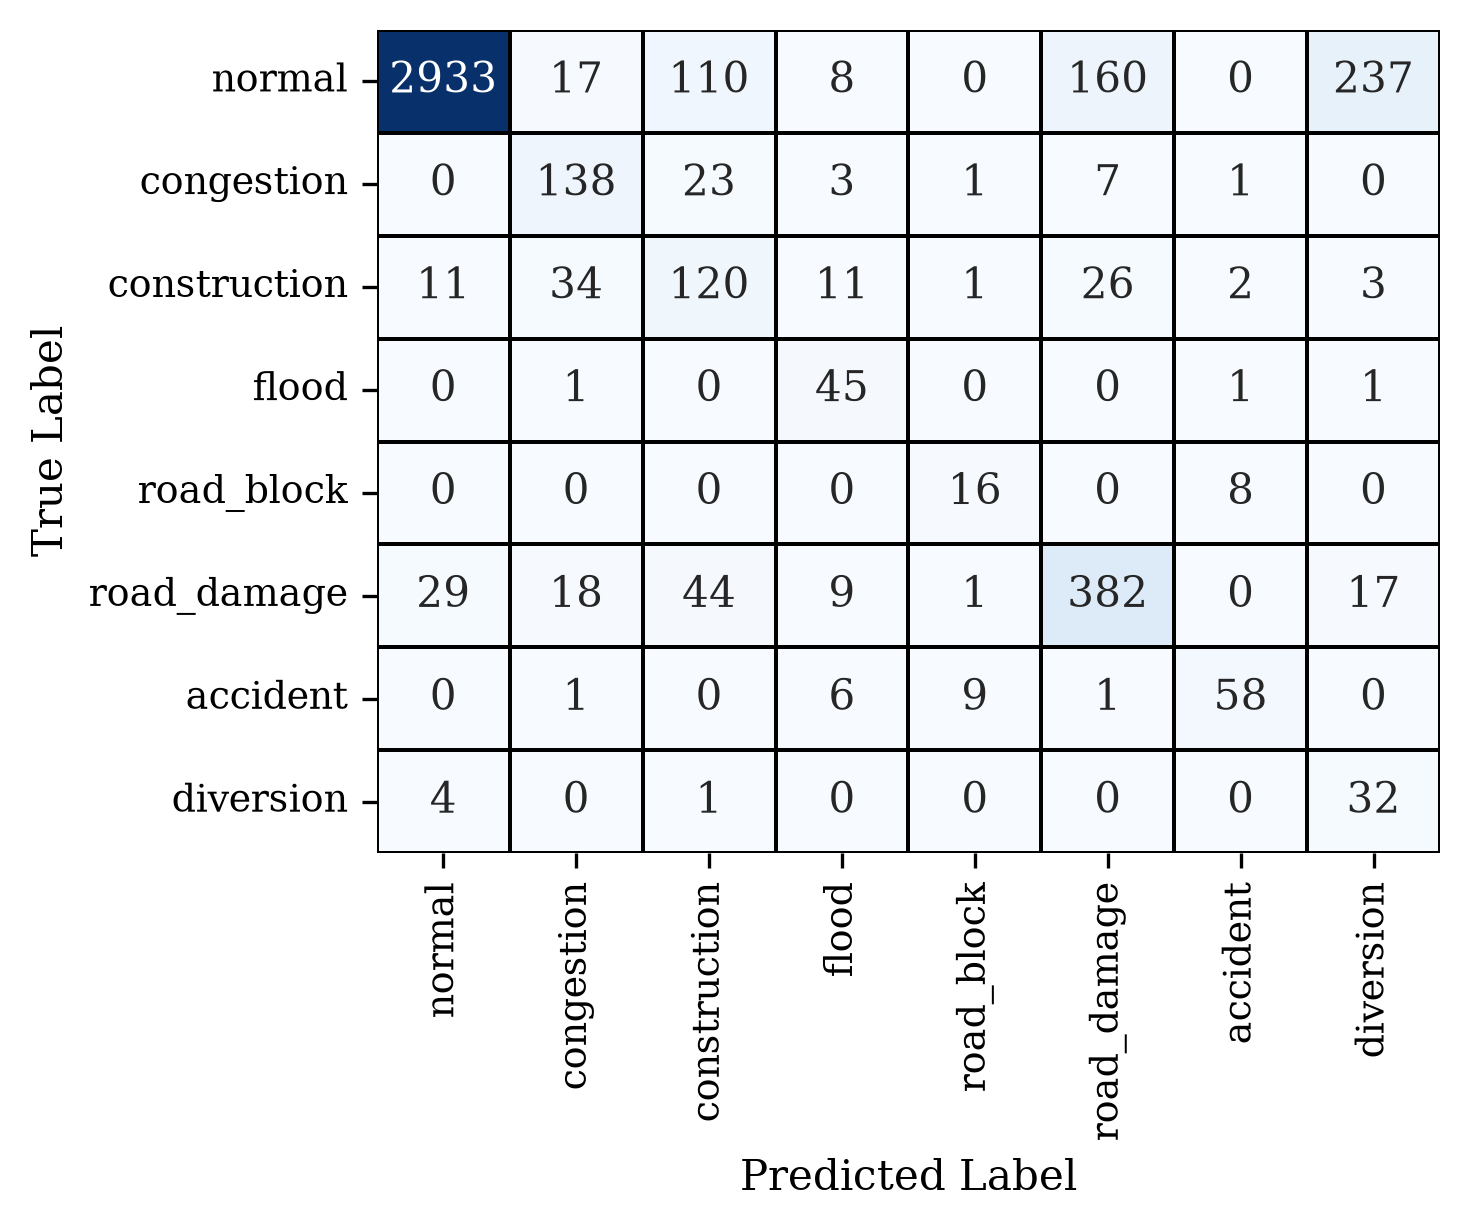
\includegraphics[width=0.9\linewidth]{figures/fig8_confusion_matrix}
  \caption{Confusion matrix for the AdaptiveFedAvg model on the held-out test set across eight traffic anomaly categories. Strong diagonal dominance confirms high classification accuracy. Minor misclassification between rare classes (\texttt{flood}, \texttt{diversion}) stems from class imbalance in local edge partitions.}
  \label{fig:confusion_matrix}
\end{figure}

\subsection{Class Distribution and Imbalance Impact}

The class distribution of the 30,195 synthetic dataset samples across 8 anomaly categories is depicted in Fig.~\ref{fig:class_distribution}. The dataset exhibits severe class imbalance: \texttt{normal} traffic comprises 76.5\% of samples, whereas minority classes such as \texttt{flood} (0.8\%) and \texttt{diversion} (0.6\%) represent less than 1\% of local observations.

\begin{figure}[htbp]
  \centering
  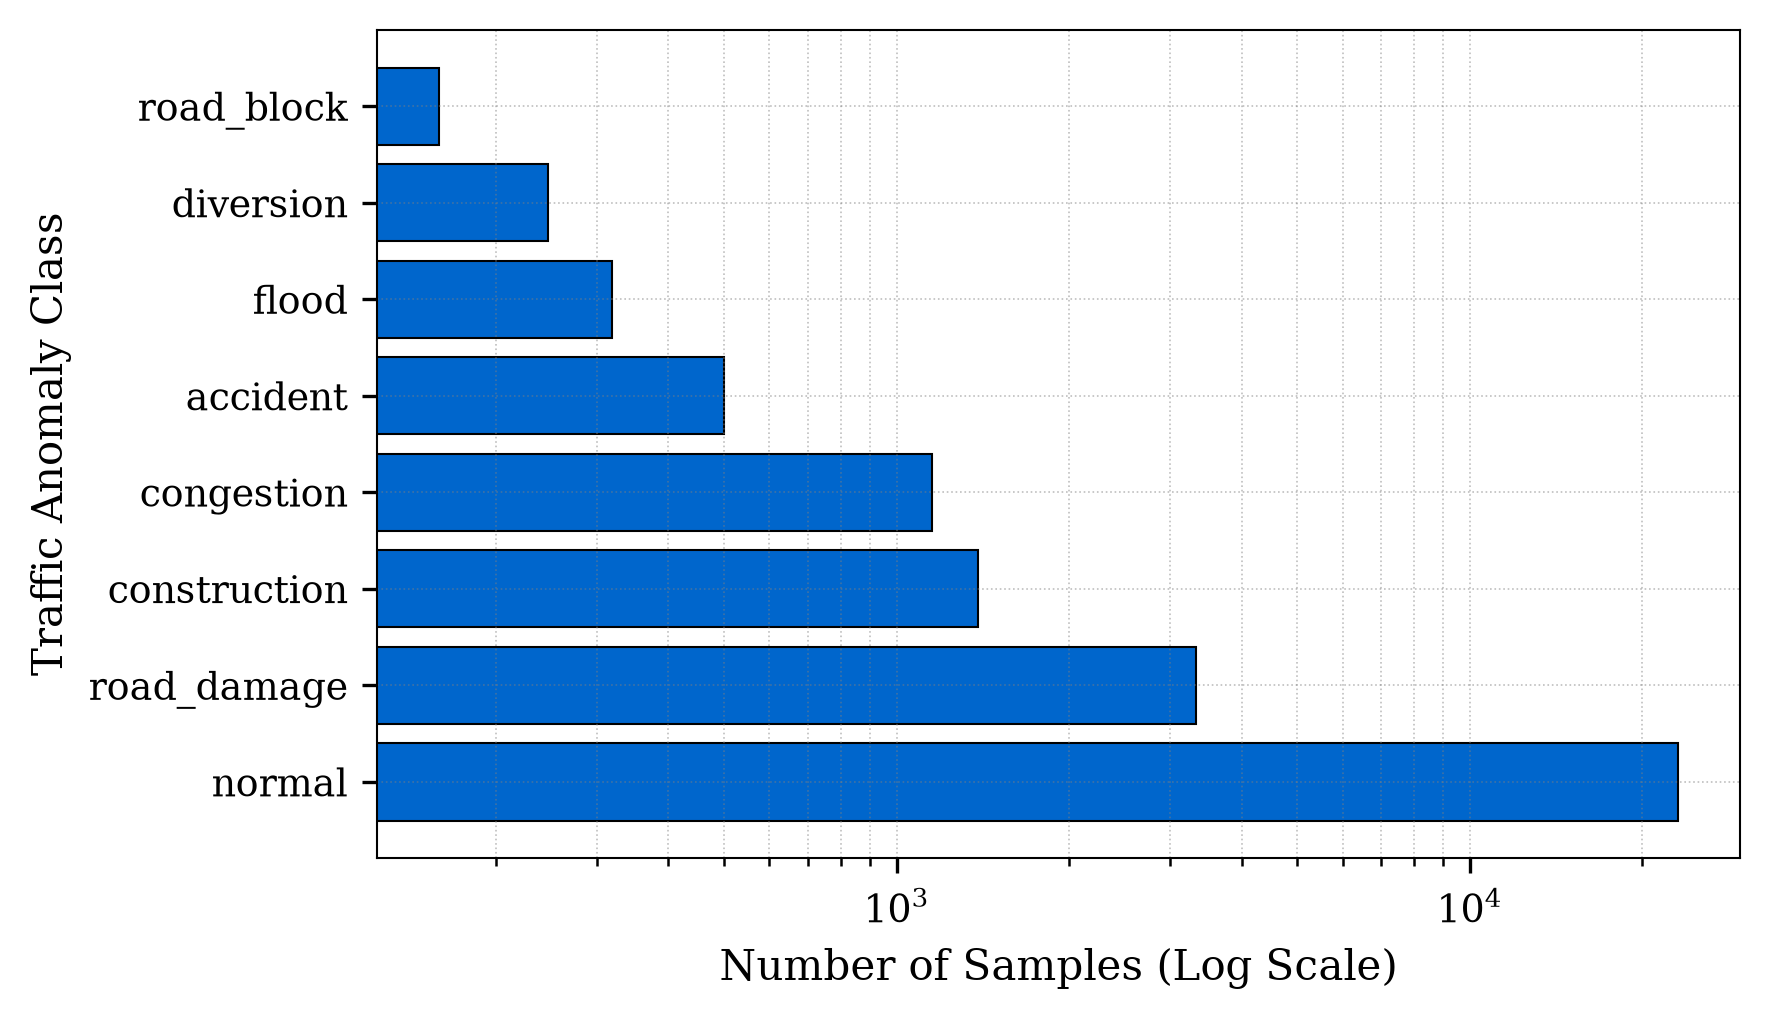
\includegraphics[width=\linewidth]{figures/fig9_class_distribution}
  \caption{Synthetic dataset class distribution across eight anomaly categories (30,195 total samples). Severe class imbalance---where \texttt{normal} dominates 76.5\% of data while minority classes fall below 1\%---motivates the bounded rarity bonus $\rho_k$ in AdaptiveFedAvg (Eq.~\ref{eq:adaptivefedavg_weight}).}
  \label{fig:class_distribution}
\end{figure}

The rarity bonus factor $\rho_k = 1.0 + \beta \cdot f_{rare}^k$ in AdaptiveFedAvg specifically counters this imbalance by inflating the aggregation weight of clients holding rare anomaly observations, ensuring minority class signatures are preserved during global parameter averaging.

\subsection{Latency and Communication Overhead}

Table~\ref{tab:latency_communication} details the inference latency and communication bandwidth metrics. The EventClassifierMLP's 3,240 parameters yield a per-round weight payload of exactly $3240 \times 4 = 12{,}960$ bytes (12.96\,KB) per client. Across 8 clients, total upload bandwidth per round is 207.36\,KB---well within V2X communication bounds.

\begin{table}[htbp]
\centering
\caption{Systems-Level Benchmarking and Communication Costs}
\label{tab:latency_communication}
\resizebox{\linewidth}{!}{%
\begin{tabular}{ll}
\toprule
\textbf{Systems Benchmark Metric} & \textbf{Empirical Measurement} \\
\midrule
Average Edge Inference Latency    & 0.2069 ms / sample (CPU) \\
Per-Client Model Upload Payload   & 12.96 KB / round ($3{,}240 \times 4$ bytes) \\
Per-Client Model Download Payload & 12.96 KB / round \\
Total Upload Bandwidth (8 Clients)& 207.36 KB / round \\
Cumulative Client Upload Bandwidth     & 6.22 MB (30 rounds $\times$ 8 clients) \\
\bottomrule
\end{tabular}%
}
\end{table}


The average inference latency across 1,000 measurement iterations is 0.2069\,ms on a standard CPU, confirming that the deployment-aware preprocessing logic (zero-imputation and OOD threshold checking) introduces negligible overhead.

\subsection{Discussion}

Three primary insights summarize the experimental evaluation:

\textbf{Federated regularization.} Decentralized training across 8 edge partitions acts as an implicit regularizer, preventing global model saturation on majority classes.

\textbf{Adaptive weighting utility.} The four-factor AdaptiveFedAvg weighting (Eq.~\ref{eq:adaptivefedavg_weight}) matches standard FedAvg under controlled conditions while offering theoretical safeguards against sensor degradation.

\textbf{Real-time edge feasibility.} The 0.2069\,ms inference latency and 12.96\,KB communication payload satisfy V2X operational constraints. Qualitative baseline comparisons and asymptotic bounds are detailed in Table~\ref{tab:methods_comparison} and Table~\ref{tab:computational_complexity}.

\begin{table*}[htbp]
\centering
\caption{Qualitative Architectural Comparison with Existing Federated and Edge Frameworks}
\label{tab:methods_comparison}
\resizebox{0.95\textwidth}{!}{%
\begin{tabular}{lcccccc}
\toprule
\textbf{Method} & \textbf{Privacy-Preserving} & \textbf{Adaptive Aggregation} & \textbf{OOD Detection} & \textbf{Deployment-Aware} & \textbf{Low Communication} & \textbf{Edge-Optimized} \\
\midrule
FedAvg \cite{McMahan_2017}     & \checkmark & $\times$    & $\times$    & $\times$    & \checkmark & \checkmark \\
FedAdam \cite{Yang_2024}    & \checkmark & \checkmark & $\times$    & $\times$    & \checkmark & \checkmark \\
FedYogi \cite{Yang_2024}    & \checkmark & \checkmark & $\times$    & $\times$    & \checkmark & \checkmark \\
\textbf{FedRouteAI (ours)} & \textbf{\checkmark} & \textbf{\checkmark} & \textbf{\checkmark} & \textbf{\checkmark} & \textbf{\checkmark} & \textbf{\checkmark} \\
\bottomrule
\end{tabular}%
}
\end{table*}


\begin{table}[htbp]
\centering
\caption{Computational Complexity and Resource Bounds}
\label{tab:computational_complexity}
\resizebox{\linewidth}{!}{%
\begin{tabular}{lll}
\toprule
\textbf{Phase / Component} & \textbf{Time Complexity} & \textbf{Memory / Payload} \\
\midrule
Historical Feature Scaling & $\mathcal{O}(d_{raw})$ & $\mathcal{O}(1)$ query overhead \\
Edge MLP Inference & $\mathcal{O}(L \cdot d_{mlp})$ & $3,240$ parameters ($\approx 12.96$ KB) \\
Local Training Epoch & $\mathcal{O}(E \cdot N_k \cdot d_{mlp})$ & Batch size 32 tensors \\
Adaptive Weight Calculation & $\mathcal{O}(1)$ per client & 4 scalar floats \\
Federated Weight Payload & $\mathcal{O}(|\theta|)$ & $12.96$ KB upload / download \\
Server Aggregation Round & $\mathcal{O}(|\mathcal{K}| \cdot |\theta|)$ & $207.36$ KB total network \\
\bottomrule
\end{tabular}%
}
\end{table}


\subsubsection{Limitations and Future Work}

The primary limitation is reliance on synthetic data; physical edge deployment will involve real-world packet drops and hardware noise. Future work includes evaluating hardware deployments on physical roadside units (RSUs) and incorporating differential privacy guarantees.

\section{Conclusion}
\label{sec:conclusion}

Reliable, real-time traffic anomaly detection in intelligent transportation systems is frequently hindered by decentralized data silos, extreme class imbalance, and the strict hardware constraints of vehicular edge nodes. This paper presented FedRouteAI, a federated learning framework that pairs a deployment-aware inference pipeline with an adaptive aggregation strategy to address these challenges. The core methodological contributions include a federated architecture that preserves data privacy across distinct regional clients, a historical feature engineering module for localized normalization, the four-factor AdaptiveFedAvg aggregation algorithm, and a deployment-aware inference mechanism relying on zero-imputation and dynamic Out-of-Distribution (OOD) warnings.

Under the evaluated synthetic dataset, the federated approaches achieved higher generalization performance than the centralized baseline. AdaptiveFedAvg's performance was comparable to standard FedAvg, with only marginal differences in global accuracy and Macro F1, which suggests that standard, dataset-proportional aggregation already performs robustly in stable deployment environments. Systems-level benchmarking additionally shows that the lightweight Multi-Layer Perceptron architecture operates with low inference latency and minimal communication overhead, meeting the latency and communication requirements evaluated in this study and remaining compatible with real-time edge deployment scenarios.

Despite these promising indications, several limitations must be acknowledged. The experimental evaluation relied entirely on a synthetic dataset and a simulated federated environment, which limits the validation of the system under true physical conditions, and it was constrained to a single MLP architecture that was not tested against the severe, erratic packet drops typical of physical edge sensors. Future work should evaluate the framework using larger and more heterogeneous federated deployments, investigate more advanced learning architectures (e.g., Graph Neural Networks or Transformer-based models), and validate the system under real roadside infrastructure.


\balance
\bibliographystyle{IEEEtran}
\bibliography{references}

\end{document}
